%% GABARIT POUR MÉMOIRE STANDARD
%%
%% Consulter la documentation de la classe ulthese pour une
%% description détaillée de la classe, de ce gabarit et des options
%% disponibles.
%%
%% [Ne pas hésiter à supprimer les commentaires après les avoir lus.]
%%
%% Déclaration de la classe avec le type de grade
%%   [l'un de MATDR, MArch, MA, LLM, MErg, MMus, MPht, MSc, MScGeogr,
%%    MServSoc, MPsEd]
%% et les langues les plus courantes. Le français sera la langue par
%% défaut du document.
\documentclass[projet,english,french]{ulthese}
  %% Encodage utilisé pour les caractères accentués dans les fichiers
  %% source du document. Les gabarits sont encodés en UTF-8. Inutile
  %% avec XeLaTeX, qui gère Unicode nativement.
  \ifxetex\else \usepackage[utf8]{inputenc} \fi
  
  %% Charger ici les autres paquetages nécessaires pour le document.
  %% Quelques exemples; décommenter au besoin.
  \usepackage{amsmath}       % recommandé pour les mathématiques
  %\usepackage{icomma}        % gestion de la virgule dans les nombres
  \usepackage{tikz}
  \usepackage{xspace}
  \usepackage{fvextra}
  \usepackage{listings}
  \usepackage{adjustbox}
  \usepackage{xcolor}

\definecolor{codegreen}{rgb}{0,0.6,0}
\definecolor{codegray}{rgb}{0.5,0.5,0.5}
\definecolor{codepurple}{rgb}{0.58,0,0.82}
\definecolor{backcolour}{rgb}{0.95,0.95,0.92}
  %% Configuration de listings
\lstset{language = R,
		basicstyle = \footnotesize\ttfamily\NoAutoSpacing,
		extendedchars = true,
		showstringspaces = false,
		frame = t,
		xleftmargin = 3.4pt,
		numbers = left,
		backgroundcolor=\color{backcolour},   
    	commentstyle=\color{codegreen},
    	numberstyle=\tiny\color{codegray},
    	breakatwhitespace=false,         
   	 	breaklines=true,                 
    	captionpos=t,                    
    	keepspaces=true,                   
    	numbersep=5pt,                  
    	showspaces=false,
    	showtabs=false}
		
\renewcommand{\lstlistingname}{Code}

\lstset{literate=
  {á}{{\'a}}1 {é}{{\'e}}1 {í}{{\'i}}1 {ó}{{\'o}}1 {ú}{{\'u}}1
  {Á}{{\'A}}1 {É}{{\'E}}1 {Í}{{\'I}}1 {Ó}{{\'O}}1 {Ú}{{\'U}}1
  {à}{{\`a}}1 {è}{{\`e}}1 {ì}{{\`i}}1 {ò}{{\`o}}1 {ù}{{\`u}}1
  {À}{{\`A}}1 {È}{{\'E}}1 {Ì}{{\`I}}1 {Ò}{{\`O}}1 {Ù}{{\`U}}1
  {ä}{{\"a}}1 {ë}{{\"e}}1 {ï}{{\"i}}1 {ö}{{\"o}}1 {ü}{{\"u}}1
  {Ä}{{\"A}}1 {Ë}{{\"E}}1 {Ï}{{\"I}}1 {Ö}{{\"O}}1 {Ü}{{\"U}}1
  {â}{{\^a}}1 {ê}{{\^e}}1 {î}{{\^i}}1 {ô}{{\^o}}1 {û}{{\^u}}1
  {Â}{{\^A}}1 {Ê}{{\^E}}1 {Î}{{\^I}}1 {Ô}{{\^O}}1 {Û}{{\^U}}1
  {Ã}{{\~A}}1 {ã}{{\~a}}1 {Õ}{{\~O}}1 {õ}{{\~o}}1
  {œ}{{\oe}}1 {Œ}{{\OE}}1 {æ}{{\ae}}1 {Æ}{{\AE}}1 {ß}{{\ss}}1
  {ű}{{\H{u}}}1 {Ű}{{\H{U}}}1 {ő}{{\H{o}}}1 {Ő}{{\H{O}}}1
  {ç}{{\c c}}1 {Ç}{{\c C}}1 {ø}{{\o}}1 {å}{{\r a}}1 {Å}{{\r A}}1
  {€}{{\euro}}1 {£}{{\pounds}}1 {«}{{\guillemotleft}}1
  {»}{{\guillemotright}}1 {ñ}{{\~n}}1 {Ñ}{{\~N}}1 {¿}{{?`}}1
}
  %% Utilisation d'une autre police de caractères pour le document.
  %% - Sous LaTeX
  \usepackage{mathpazo}      % texte et mathématiques en Palatino
  %\usepackage{mathptmx}
  \usepackage{amsfonts}      % texte et mathématiques en Times
  %% - Sous XeLaTeX
  %\setmainfont{TeX Gyre Pagella}      % texte en Pagella (Palatino)
  %\setmathfont{TeX Gyre Pagella Math} % mathématiques en Pagella (Palatino)
  %\setmainfont{TeX Gyre Termes}       % texte en Termes (Times)
  %\setmathfont{TeX Gyre Termes Math}  % mathématiques en Termes (Times)

  %% Options de mise en forme du mode français de babel. Consulter la
  %% documentation du paquetage babel pour les options disponibles.
  %% Désactiver (effacer ou mettre en commentaire) si l'option
  %% 'nobabel' est spécifiée au chargement de la classe.
  \frenchbsetup{%
  	StandardLists=true,
    StandardItemizeEnv=true,       % format standard des listes
    ThinSpaceInFrenchNumbers=true, % espace fine dans les nombres
    og=«, fg=»                         % caractères « et » sont les guillemets
  }


  %% Style de la bibliographie.
 \bibliographystyle{francais}

  %% Composition de la page frontispice. Remplacer les éléments entre < >.
  %% Supprimer les caractères < >. Couper un long titre ou un long
  %% sous-titre manuellement avec \\.
  \titre{Réseau de neurones en actuariat}
  % \titre{Ceci est un exemple de long titre \\
  %   avec saut de ligne manuel}
  % \soustitre{Sous-titre le cas échéant}
  % \soustitre{Ceci est un exemple de long sous-titre \\
  %   avec saut de ligne manuel}
  \auteur{Nicolas Bellemare}
  \programme{Baccalauréat en actuariat}
  \direction{Marie-Pier Côté, directrice de recherche}
  % \codirection{<Prénom Nom>, <codirecteur ou codirectrice> de recherche}
  % \codirection{<Prénom Nom>, <codirecteur ou codirectrice> de recherche \\
  %              <Prénom Nom>, <codirecteur ou codirectrice> de recherche}

  %% Les commandes ci-dessous servent uniquement pour la création
  %% d'une page de titre (interdite lors du dépôt à la FESP).
   \annee{2020}

\begin{document}

\frontmatter                    % pages liminaires

\pagetitre                  % production de la page titre
           % résumé français
\cleardoublepage

\tableofcontents                % production de la TdM
\cleardoublepage

\listoftables                   % production de la liste des tableaux
\cleardoublepage

\listoffigures                  % production de la liste des figures
\cleardoublepage



\mainmatter                     % corps du document

\chapter*{Introduction}         % ne pas numéroter
\label{chap:introduction}       % étiquette pour renvois
\phantomsection\addcontentsline{toc}{chapter}{\nameref{chap:introduction}} % inclure dans TdM

<Texte de l'introduction. La thèse ou le mémoire devrait normalement
débuter par une introduction. Celle-ci est traitée comme un chapitre
normal, sauf qu'elle n'est pas numérotée.>
          % introduction
\chapter{Théorie des réseaux de neurones}     
\label{chap:RN}                   

\section{Apprentissage supervisé}
\label{sec:RN:ML}

La section présente est basée sur le chapitre 2 de \citet{james2013introduction} et le chapitre 2 de \citet{Hastie/etal:2009}.

Les réseaux de neurones sont des modèles qui peuvent s'appliquer tant à l'apprentissage supervisé qu'à l'apprentissage non-supervisé. On résume dans cette section les bases de l'apprentissage supervisé pour la suite.

Soit $X=\left(X_1, \dots X_p \right)$, un vecteur de $p$ variables aléatoires et $Y$, une variable que l'on veut prédire. On suppose qu'il existe une relation entre $Y$ et $X$ telle que,

\begin{align*}
Y = f(X) + \epsilon,
\end{align*} 

où $f$ est une fonction quelconque et $\epsilon$ est un terme d'erreur qui est indépendant de $X$. L'apprentissage supervisé vise à estimer $f$ pour pouvoir prédire et/ou expliquer $Y$ à partir de $X$. On veut utiliser les données pour estimer une fonction $f$ qui soit utile, c'est-à-dire, une fonction qui permet de bien estimer $Y$ à partir de nouvelles données. 

Un algorithme d'apprentissage supervisé est capable de modifier ses paramètres internes en réponse à une fonction objective. En d'autres termes, il apprend à partir des erreurs commises.  La fonction objective mesure donc la différence entre la prédiction, $\hat{f}(x)$, et la vraie valeur de $Y$. On dénote cette fonction par 

\begin{align*}
\mathcal{L} \left( Y, \hat{f}(X) \right)= \left( \hat{f}(X) - Y\right)^2.
\end{align*}

\subsection{Compromis biais-variance}
\label{subsec:RN:ML:biais-var}

Un des enjeux principaux en apprentissage statistique est le compromis biais-variance. On veut un modèle qui soit le plus précis possible tout en étant le moins variable possible. Par contre, lorsqu'on diminue le biais, la variance de l'estimateur finit toujours par augmenter: on doit trouver le compromis. On illustre cet enjeu par l'erreur quadratique espérée:

\begin{align*}\mathrm{E}\left[\left\{Y_{0}-\hat{f}\left(X\right)\right\}^{2}\right]=\operatorname{Biais}^{2}\left\{\hat{f}\left(X\right)\right\}+\operatorname{var}\left\{\hat{f}\left(X\right)\right\}+ \sigma^{2},
\end{align*}
où $\sigma^2=\operatorname{var}\left(\epsilon\right)$, l'erreur irréductible.

On ne peut pas diminuer l'erreur irréductible, comme son nom l'indique, puisqu'elle fait partie de tout processus aléatoire. Toutefois, on peut diminuer l'erreur réductible (biais + variance) en diminuant ou en augmentant la complexité du modèle. La complexité du modèle se traduit par le nombre de paramètres qu'il faut estimer. Plus on a de paramètres, plus le modèle est en mesure de faire des prédictions exactes sur les données d'entrainement. En revanche, la variance sera plus élevée, car le modèle aura appris les caractéristiques  des observations qui sont propres à celles-ci. 

Pour être en mesure de surveiller le compromis, on sépare les données en trois échantillons distincts: l'échantillon d'entrainement, l'échantillon de validation et l'échantillon de test. L'échantillon d'entrainement $\mathcal{D}$ est celui sur lequel on entraine le modèle; il sert à ajuster les paramètres. L'échantillon de test $\mathcal{T}$ permet de mesurer la performance du modèle et ainsi le comparer avec d'autres. L'échantillon de validation $\mathcal{V}$ permet de faire la sélection d'hyperparamètres et c'est à partir de celui-ci qu'on surveille si le modèle ne surajuste pas les données d'entrainement. 

\begin{figure}[h]
\centering
\caption{\label{fig:ErrPredVsComplex}Erreur de prédiction en fonction de la complexité du modèle}
\includegraphics[height=8cm,width=10cm]{Rplot_prederror_complexité}
\end{figure}

La \autoref{fig:ErrPredVsComplex} montre un example de l'erreur de prédiction en fonction de la complexité d'un modèle. On voit que plus la complexité augmente, plus l'erreur de prédiction sur les données d'entrainement diminue. On remarque, aussi, que l'erreur de prédiction sur les données de validation diminue lorsqu'on augmente la complexité pour ensuite augmenter. Lorsque le modèle atteint le point où l'erreur de prédiction sur l'échantillon de validation augmente, on dit que le modèle surajuste l'échantillon d'entrainement. Il ne généralise pas bien pour des données qu'il n'a pas vu. L'objectif devient donc de trouver une combinaison des paramètres à estimer et de la complexité du modèle pour minimiser la fonction objective sur l'échantillon de validation.

\section{Architecture d'un réseau de neurones}
\label{sec:RN:architecture}

Malgré qu'il existe plusieurs types de réseau de neurones, la section présente ainsi que l'analyse de données subséquente sont basées sur la forme la plus simple de réseau de neurones, soit le perceptron ou réseau de neurones à propagation directe (« feedforward neural network »). Il existe deux formes de perceptron: le perceptron simple et le perceptron multicouche.  La différence entre les deux formes réside dans le nombre de couche cachée. Le perceptron simple a une seule couches cachées, tandis que le perceptron multicouche en a plusieurs. Pour bien comprendre le perceptron, on compare son fonctionnement avec des modèles plus simples. On illustre les modèles de régression linéaire simple et multiple et le modèle de régression logistique pour expliquer la progression qui nous amènera au réseau de neurones.

\def\layersep{2.5cm}

\begin{figure}[h]
\centering
\caption{\label{fig:reglin}Modèle de régression linéaire simple}
\begin{tikzpicture}[shorten >=1pt,->,draw=black!50, node distance=\layersep]
    \tikzstyle{every pin edge}=[<-,shorten <=1pt]
    \tikzstyle{neuron}=[circle,fill=black!25,minimum size=17pt,inner sep=0pt]
    \tikzstyle{input neuron}=[neuron, fill=green!50];
    \tikzstyle{output neuron}=[neuron, fill=red!50];
    \tikzstyle{hidden neuron}=[neuron, fill=blue!50];
    \tikzstyle{bias}=[neuron, fill=yellow!50];
    \tikzstyle{annot} = [text width=4em, text centered]

    % Draw the input layer nodes
        \node[input neuron] (I-1) at (0,-1) {$x$};
        
	%Bias node
	\node[bias] (B1) at (0.5*\layersep,-0.5 cm) {$b$};	        

    % Draw the hidden layer nodes
   	\node[hidden neuron] (S-1) at (\layersep,-1 cm) {$\sum$};

	
	% Draw the output layer node, first the sum then the response
	\node[output neuron] (O) at (2*\layersep,-1 cm) {$\hat{y}$};

    
   

    % Connect every node in the input layer with every node in the
    % sum layer.
            \path (I-1) edge (S-1);
	
	% Connect les biais avec les sommes
            \path (B1) edge (S-1);
            
	% Connect every node in the sum layer with every node in the
    % hidden layer.
            
    % Connect every node in the hidden layer with the output sum layer

        \path (S-1) edge (O);
	
	
    % Annotate the layers
    \node[annot,below of=I-1, node distance=1cm] (i1) {Variable exogène};
    \node[annot,right of=i1, node distance=\layersep] (hid1) {Sommation};
    \node[annot,right of=hid1,node distance=\layersep] {Variable réponse};
\end{tikzpicture}
\end{figure}

Un modèle de régression linéaire simple est une somme de la variable exogène. On suppose que la relation entre $Y$ et $X$ est de la forme suivante:
\begin{align*}
Y = b+\omega X + \epsilon.
\end{align*}
On estime $Y$ par
\begin{align*}
\hat{Y} = \hat{f} (X) = \hat{b}+\hat{\omega} X.
\end{align*}
Ce modèle utilise l'information qui est contenue dans la variable exogène pour prédire la variable réponse. Pour ce faire, on calcule $\hat{b}$ et $\hat{\omega}$ de façon à minimiser l'erreur quadratique de prévision.  
On illustre ce modèle à l'aide 
de la \autoref{fig:reglin}. La partie verte de la figure illustre l'information qui entre dans le modèle, la partie bleue est le traitement de l'information et la partie rouge est la prévision du modèle. On voit que la partie bleue est en fait la fonction $\hat{f}$. Le terme de la partie jaune est le biais. 

\begin{figure}[h]
\centering
\caption{\label{fig:reg:lin:mult}Modèle de régression multiple}
\begin{tikzpicture}[shorten >=1pt,->,draw=black!50, node distance=\layersep]
    \tikzstyle{every pin edge}=[<-,shorten <=1pt]
    \tikzstyle{neuron}=[circle,fill=black!25,minimum size=17pt,inner sep=0pt]
    \tikzstyle{input neuron}=[neuron, fill=green!50];
    \tikzstyle{output neuron}=[neuron, fill=red!50];
    \tikzstyle{hidden neuron}=[neuron, fill=blue!50];
    \tikzstyle{bias}=[neuron, fill=yellow!50];
    \tikzstyle{annot} = [text width=4em, text centered]

    % Draw the input layer nodes
    \foreach \name / \y in {1,...,3}
    % This is the same as writing \foreach \name / \y in {1/1,2/2,3/3,4/4}
        \node[input neuron] (I-\name) at (0,-\y) {$x_{\y}$};
        
	%Bias node
	\node[bias] (B1) at (0.5*\layersep,-0.5 cm) {$b$};	        

    % Draw the hidden layer nodes
    \node[hidden neuron] (S-1) at (\layersep,-2 cm) {$\sum$};
	
	% Draw the output layer node, first the sum then the response    	
    	\node[output neuron] (O) at (2*\layersep,-2 cm) {$\hat{y}$};

    
   

    % Connect every node in the input layer with every node in the
    % sum layer.
    \foreach \source in {1,...,3}
            \path (I-\source) edge (S-1);
	
	% Connect les biais avec les sommes
    \path (B1) edge (S-1);
            
	% Connect every node in the sum layer with every node in the
    % hidden layer.
    \path (S-1) edge (O);

	
	
    % Annotate the layers
    \node[annot,below of=I-3, node distance=1cm] (i1) {Variables exogènes};
    \node[annot,right of=i1, node distance=\layersep] (hid1) {Sommation};
    \node[annot,right of=hid1,node distance=\layersep] {Variable réponse};
\end{tikzpicture}
\end{figure} 

Dans le cas de la régression linéaire multiple, on a plusieurs variables exogènes. On fait une sommation pondérée de toutes ces variables pour pouvoir prédire la variable réponse. La relation entre Y et X est
\begin{align*}
Y = b + \sum_{i=1}^n \omega_{i} X_i + \epsilon.
\end{align*}

On estime Y par

\begin{align*}
\hat{Y} = \hat{f} (X) = \hat{b}+\sum_{i=1}^n \hat{\omega}_{i} X_i.
\end{align*}

 La \autoref{fig:reg:lin:mult} illustre un cas avec 3 variables exogènes. On y voit le même mécanisme 
qu'avec la régression linéaire simple, c'est-à-dire, on combine l'information, on la traite et puis on prédit un résultat. La différence est que l'information a plus d'une dimension. On doit donc estimer un paramètre pour chaque variable exogène et un paramètre pour le biais. Il s'en dégage une structure qui est bien présente dans les modèles d'apprentissage statistique. 


\begin{figure}[h]
\centering
\caption{\label{fig:reg:log}Régression logistique}
\begin{tikzpicture}[shorten >=1pt,->,draw=black!50, node distance=\layersep]
    \tikzstyle{every pin edge}=[<-,shorten <=1pt]
    \tikzstyle{neuron}=[circle,fill=black!25,minimum size=17pt,inner sep=0pt]
    \tikzstyle{input neuron}=[neuron, fill=green!50];
    \tikzstyle{output neuron}=[neuron, fill=red!50];
    \tikzstyle{hidden neuron}=[neuron, fill=blue!50];
    \tikzstyle{bias}=[neuron, fill=yellow!50];
    \tikzstyle{annot} = [text width=4em, text centered]

    % Draw the input layer nodes
    \foreach \name / \y in {1,...,3}
    % This is the same as writing \foreach \name / \y in {1/1,2/2,3/3,4/4}
        \node[input neuron] (I-\name) at (0,-\y) {$x_{\y}$};
        
	%Bias node
	\node[bias] (B1) at (0.5*\layersep,-0.5 cm) {$b$};	        

    % Draw the hidden layer nodes

    \node[hidden neuron] (S-1) at (\layersep,-2 cm) {$\sum$};
            
    \node[hidden neuron] (H-1) at (2*\layersep,-2 cm) {$\phi$};

	
	% Draw the output layer node, first the sum then the response
    	
    	\node[output neuron] (O) at (3*\layersep,-2 cm) {$\hat{y}$};

    
   

    % Connect every node in the input layer with every node in the
    % sum layer.
    \foreach \source in {1,...,3}
            \path (I-\source) edge (S-1);
	
	% Connect les biais avec les sommes
            \path (B1) edge (S-1);
            
	% Connect every node in the sum layer with every node in the
    % hidden layer.
            \path (S-1) edge (H-1);
            
    % Connect every node in the hidden layer with the output sum layer
        \path (H-1) edge (O);
	
	
    % Annotate the layers
    \node[annot,below of=I-3, node distance=1cm] (i1) {Variables exogènes};
    \node[annot,right of=i1, node distance=\layersep + 0.5*\layersep] (hid1) {Fonction de lien};
    \node[annot,right of=hid1,node distance=1.5*\layersep] {Variable réponse};
\end{tikzpicture}
\end{figure}

La régression logistique, quant à elle, ajoute une transformation non-linéaire à la combinaison linéaire des variables exogènes. Ainsi, la variable prédite peut être contenue dans l'espace $[0,1]$. La \autoref{fig:reg:log} ajoute donc $\phi$ au traitement de l'information. Le modèle est

\begin{align*}
Y = \frac{e^{b+ \sum_{i=1}^n \omega_{i} X_i}}{1+e^{b+ \sum_{i=1}^n \omega_{i} X_i}}.
\end{align*}

La relation entre Y et X est ainsi non-linéaire. On peut voir la régression logistique comme étant un réseau de neurones avec une seule couche cachée et un seul neurone dans la couche cachée. 

\begin{figure}[h]
	\centering
	\caption[Réseau de neurones avec une couche cachée]{\label{fig:NNsimple}Réseau de neurones avec une couche cachée\footnotemark} 
\begin{tikzpicture}[shorten >=1pt,->,draw=black!50, node distance=\layersep]
    \tikzstyle{every pin edge}=[<-,shorten <=1pt]
    \tikzstyle{neuron}=[circle,fill=black!25,minimum size=17pt,inner sep=0pt]
    \tikzstyle{input neuron}=[neuron, fill=green!50];
    \tikzstyle{output neuron}=[neuron, fill=red!50];
    \tikzstyle{hidden neuron}=[neuron, fill=blue!50];
    \tikzstyle{bias}=[neuron, fill=yellow!50];
    \tikzstyle{annot} = [text width=4em, text centered]

    % Draw the input layer nodes
    \foreach \name / \y in {1,...,3}
    % This is the same as writing \foreach \name / \y in {1/1,2/2,3/3,4/4}
        \node[input neuron] (I-\name) at (0,-\y) {$x_{\y}$};
        
	%Bias node
	\node[bias] (B1) at (0.5*\layersep,-0.5 cm) {$b^{1}$};	        

    % Draw the hidden layer nodes
    \foreach \name / \y in {1,...,2}
        \path[yshift=-0.5cm]
            node[hidden neuron] (S-\name) at (\layersep,-\y cm) {$\sum$};
            
    \foreach \name / \y in {1,...,2}
        \path[yshift=-0.5cm]
            node[hidden neuron] (H-\name) at (2*\layersep,-\y cm) {$\phi_{\y}$};

	% Draw les biais pour la somme output
	\node[bias] (B2) at (2.5*\layersep,-0.5 cm) {$b^{2}$};	
	
	% Draw the output layer node, first the sum then the response
    	\node[output neuron] (OS) at (3*\layersep,-2 cm) {$\sum$};
    	
    	\node[output neuron] (O) at (4*\layersep,-2 cm) {$\hat{y}$};

    
   

    % Connect every node in the input layer with every node in the
    % sum layer.
    \foreach \source in {1,...,3}
        \foreach \dest in {1,...,2}
            \path (I-\source) edge (S-\dest);
	
	% Connect les biais avec les sommes
	\foreach \dest in {1,...,2}
            \path (B1) edge (S-\dest);
            
	% Connect every node in the sum layer with every node in the
    % hidden layer.
	\foreach \source in {1,...,2}
            \path (S-\source) edge (H-\source);
            
    % Connect every node in the hidden layer with the output sum layer
    \foreach \source in {1,...,2}
        \path (H-\source) edge (OS);
	
	% Connect bias with the output sum layer
	\path (B2) edge (OS);
	
	% Connect every node in the hidden layer with the output sum layer
	\path (OS) edge (O);
	
    % Annotate the layers
    \node[annot,below of=I-3, node distance=1cm] (i1) {Couche d'entrée};
    \node[annot,right of=i1, node distance=\layersep + 0.5*\layersep] (hid1) {Couche cachée};
    \node[annot,right of=hid1,node distance=2*\layersep] {Couche de sortie};
\end{tikzpicture}
\end{figure}

\footnotetext{Ce graphique est une adaptation de la réponse de l'utilisateur \emph{gvgramazio} sur \url{https://tex.stackexchange.com/questions/153957/drawing-neural-network-with-tikz}}

Les trois exemples précédents permettent de voir que les réseaux de neurones ne sont en fait qu'une généralisation de la régression linéaire. En effet, comme le montre la \autoref{fig:NNsimple}, la partie de traitement de l'information(en bleu) est constituée de plusieurs neurones(deux neurones dans cet exemple). À chaque neurone, on combine linéairement les variables exogènes et on applique la fonction d'activation $\phi$. Ensuite, la combinaison linéaire de la réponse de chacun de ces neurones est utilisée pour prédire la variable réponse du réseau. Chaque résultat des fonctions $\phi$ deviennent à leur tour de nouvelles variables entrant dans un réseau. Illustrons ceci par un exemple.

\begin{figure}[h]
	\centering
	\caption{\label{fig:TransfoNNsimple}Décomposition d'un réseau en une suite de deux réseaux} 
\def\layersep{2cm}
\begin{tikzpicture}[shorten >=1pt,->,draw=black!50, node distance=\layersep]
    \tikzstyle{every pin edge}=[<-,shorten <=1pt]
    \tikzstyle{neuron}=[circle,fill=black!25,minimum size=17pt,inner sep=0pt]
    \tikzstyle{input neuron}=[neuron, fill=green!50];
    \tikzstyle{output neuron}=[neuron, fill=red!50];
    \tikzstyle{hidden neuron}=[neuron, fill=blue!50];
    \tikzstyle{bias}=[neuron, fill=yellow!50];
    \tikzstyle{annot} = [text width=4em, text centered]

    % Draw the input layer nodes
    \foreach \name / \y in {1,...,3}
    % This is the same as writing \foreach \name / \y in {1/1,2/2,3/3,4/4}
        \node[input neuron] (I-\name) at (0,-\y) {$x_{\y}$};
        
	%Bias node
	\node[bias] (B1) at (0.5*\layersep,-0.5 cm) {$\omega_0^{1}$};	        

    % Draw the hidden layer nodes
    \foreach \name / \y in {1,...,2}
        \path[yshift=-0.5cm]
            node[hidden neuron] (S-\name) at (\layersep,-\y cm) {$\sum$};
            
    \foreach \name / \y in {1,...,2}
        \path[yshift=-0.5cm]
            node[hidden neuron] (H-\name) at (2*\layersep,-\y cm) {$\phi_{\y}$};
            
	\foreach \name / \y in {1,...,2}
        \path[yshift=-0.5cm]
            node[input neuron] (HI-\name) at (3*\layersep,-\y cm) {$\tilde{X}_{\y}$};


	% Draw les biais pour la somme output
	\node[bias] (B2) at (3.5*\layersep,-0.5 cm) {$\omega_0^{2}$};	
	
	% Draw the output layer node, first the sum then the response
    	\node[hidden neuron] (OS) at (4*\layersep,-2 cm) {$\sum$};
    	
    	\node[output neuron] (O) at (5*\layersep,-2 cm) {$y$};

    
   

    % Connect every node in the input layer with every node in the
    % sum layer.
    \foreach \source in {1,...,3}
        \foreach \dest in {1,...,2}
            \path (I-\source) edge (S-\dest);
	
	% Connect les biais avec les sommes
	\foreach \dest in {1,...,2}
            \path (B1) edge (S-\dest);
            
	% Connect every node in the sum layer with every node in the
    % hidden layer.
	\foreach \source in {1,...,2}
            \path (S-\source) edge (H-\source);
            
    % Connect every node in the hidden layer with the output sum layer
    \foreach \source in {1,...,2}
        \path (H-\source) edge (HI-\source);
	
	\foreach \source in {1,...,2}
        \path (HI-\source) edge (OS);
	% Connect bias with the output sum layer
	\path (B2) edge (OS);
	
	% Connect every node in the hidden layer with the output sum layer
	\path (OS) edge (O);
	
    % Annotate the layers
    \node[annot,below of=I-3, node distance=1cm] (i1) {Couche d'entrée};
    \node[annot,right of=i1,node distance= 4*\layersep] (hid1) {Nouveau réseau};
    %\node[annot,right of=hid1,node distance=2*\layersep] {Couche de sortie};
\end{tikzpicture}
\end{figure}

La \autoref{fig:TransfoNNsimple} montre que les fonctions non-linéaires $\phi_j$ créent une nouvelle représentation de l'information. Cette représentation est alors combinée linéairement et traitée par un autre réseau. On voit que l'on peut reproduire cette séquence un nombre indéfini de fois. Par mesure de simplicité et pour ne pas saturer les graphiques, on résume chaque neurone par $a_j^1 = \phi_j \left(b^1 + \sum_{i=1}^n \omega_i^1 X_i \right)$, pour le $j$ième neurone de la première couche cachée, et par $a_j^l  = \phi \left( b_j^l+ \sum_{k=1}^{q_{k-1}} \omega_{j,k}^l a_k^{l-1} \right)$, pour le $j$ième neurone de la $l$ième couche cachée. On a $q_k$ neurones pour la $k$ième couche cachée. La \autoref{fig:NN:Deep2} illustre un réseau de neurones en considérant cette notation avec deux couches cachées de quatre et trois neurones, respectivement. On remarque une neurone supplémentaire directement lié à la prévision, soit $a_1^3$ dans notre exemple, ou $z_1^{l+1}$ pour un réseau avec $k$ couches cachées et une seule prédiction. Ce dernier neurone permet de faire le lien entre entre le réseau et la prévision. C'est la fonction de régression. 

\begin{figure}[h]
	\centering
	\caption{\label{fig:NN:Deep2}Réseau de neurones avec deux couches cachées} 
\def\layersep{2cm}
\begin{tikzpicture}[shorten >=1pt,->,draw=black!50, node distance=\layersep]
    \tikzstyle{every pin edge}=[<-,shorten <=1pt]
    \tikzstyle{neuron}=[circle,fill=black!25,minimum size=17pt,inner sep=0pt]
    \tikzstyle{input neuron}=[neuron, fill=green!50];
    \tikzstyle{output neuron}=[neuron, fill=red!50];
    \tikzstyle{hidden neuron}=[neuron, fill=blue!50];
    \tikzstyle{bias}=[neuron, fill=yellow!50];
    \tikzstyle{annot} = [text width=4em, text centered]

    % Draw the input layer nodes
    \foreach \name / \y in {1,...,3}
    % This is the same as writing \foreach \name / \y in {1/1,2/2,3/3,4/4}
        \path[yshift=-0.5cm] node[input neuron] (I-\name) at (0,-\y) {$x_{\y}$};
    %Première couche 4 neurones             
    \foreach \name / \y in {1,...,4}
            \node[hidden neuron] (H-\name) at (\layersep,-\y cm) {$a_{\y}^1$};
    %Deuxième couche 3 neurones
	\foreach \name / \y in {1,...,3}
        \path[yshift=-0.5cm]
            node[hidden neuron] (H2-\name) at (2*\layersep,-\y cm) {$a_{\y}^2$};
    	
    	\node[output neuron] (OA) at (3*\layersep, -2.5 cm) {$a_{1}^3$};
    	\node[output neuron] (O) at (3.5*\layersep,-2.5 cm) {$\hat{y}$};

    
   

    % Connect every node in the input layer with every node in the
    % sum layer.
    \foreach \source in {1,...,3}
        \foreach \dest in {1,...,4}
            \path (I-\source) edge (H-\dest);
	
	% Connect la première couche cachée et la deuxième
	\foreach \source in {1,...,4}
        \foreach \dest in {1,...,3}
            \path (H-\source) edge (H2-\dest);
            
    % Connect every node in the 2nd hidden layer with the output 
    \foreach \source in {1,...,3}
        \path (H2-\source) edge (OA);
	
	\path (OA) edge (O);	
	
    % Annotate the layers
    \node[annot,below of=I-3, node distance=1.5cm] (i1) {Couche d'entrée};
    \node[annot,right of=i1,node distance= 1.5*\layersep] (hid1) {Couches cachées};
    \node[annot,right of=hid1,node distance=1.75*\layersep] {Couche de sortie};
\end{tikzpicture}
\end{figure}

On obtient la formule suivante pour un réseau de neurones avec une couche cachée de $q_1$ neurones et avec la fonction identité pour la fonction de régression, $z_1^3(x)$:  

\begin{align*}
Y=  b^2  + \sum_{j=1}^{q_1}  \omega_{1,j}^2  \; \phi_j \left(b_j^1 + \sum_{k=1}^n \omega_{j,k}^1 \; X_k \right)
\end{align*}


\section{Phase de propagation directe(« feedforward »)}
\label{sec:RN:feedforward}

On résume la notation:

\begin{itemize}
\item $ \omega_{j,k}^1$, le poids du lien entre le $k$ème neurone de la $l-1$ème couche au $j$ème neurone de la $l$ème couche
\item $b_j^l$, le biais associé au $j$ème neurone de la $l$ème couche
\item $\phi$, une fonction d'activation quelconque
\item $a_j^l$, l'activation du $j$ème neurone de la $l$ème couche
\item $z_j^l$, l'intrant du $j$ème neurone de la $l$ème couche
\end{itemize}

On utilise une notation sous forme de matrice pour la suite.
Ainsi, on a la matrice de poids suivante pour relier la couche $l-1$ à la couche $l$

\begin{align*}
\omega^l = 
\begin{bmatrix}
\omega^l_{1,1} &\omega^l_{1,2} & \cdots &\omega^l_{1,q_l}\\
\omega^l_{2,1} &\omega^l_{2,2} & \cdots &\omega^l_{2,q_l}\\
\vdots & \vdots &\ddots & \vdots \\
\omega^l_{q_l,1} &\omega^l_{q_l,2} & \cdots &\omega^l_{q_l,q_l}\\
\end{bmatrix}.
\end{align*}

On a que 
\begin{align*}
z_j^l&= \sum_k \omega_{j,k}^1 a_j^{l-1} + b_j^l\\
\text{et}\\
z^l&= \omega^l a^{l-1} + b^l.
\end{align*}

Alors, la matrice des intrants de la $l$ème couche avec $q_l$ neurones est
\begin{align*}
z^l=
\begin{bmatrix}
z_1^l\\
\\
z_2^l\\
\vdots \\
z_{q_l}^l
\end{bmatrix}.
\end{align*}

Ainsi, on peut réécrire
\begin{align*}
a_j^l&= \phi \left( \sum_k \omega_{j,k}^1 a_j^{l-1} + b_j^l \right)\\
a^l&= \phi \left( \omega^l a^{l-1} + b^l \right).
\end{align*}

Ce qui donne pour la matrice des activations de la $l$ème couche de $q_l$ neurones

\begin{align*}
a^l=
\begin{bmatrix}
a_1^l\\
\\
a_2^l\\
\vdots \\
a_{q_l}^l
\end{bmatrix}.
\end{align*}


\section{Fonction d'activation}
\label{sec:RN:activation}

La fonction d'activation permet de créer une représentation non-linéaire de l'information.  Elle doit absolument être non-linéaire, sinon le réseau serait une combinaison linéaire de combinaisons linéaires. Elle permet ainsi d'apprendre des interactions complexes entre les variables exogènes. Les fonctions d'activation les plus communes sont

\begin{align*}
\phi(x)=
\begin{cases}
\frac{e^{x}}{1+e^{x}} &, \text{sigmoid} \\
\tanh (x) &,\text{tangente hyperbolique}\\
\mathbf{1}_{\{x \geq 0\}} &, \text{escalier} \\
x \mathbf{1}_{\{x \geq 0\}} &, \text{«Rectified Linear unit», Relu}
\end{cases}
\end{align*}

\section{Rétro-propagation(« backpropagation ») }
\label{sec:RN:back}

Cette section est inspirée de la série sur les réseaux de neurones de la page Youtube \citet{3blue1brown} et du chapitre sur le « backpropagation » de \citet{nielsen2015neural}.

On aborde maintenant le mécanisme d'apprentissage du réseau de neurone à propagation directe. On dit propagation directe(« feedforward ») puisque l'information ne fait que se propager vers l'avant. Il n'y a pas de cycle dans le modèle où l'information repasse dans une partie du réseau plusieurs fois via une boucle. Un réseau dont l'information circule de cette façon est appelé un réseau de neurones récurent. 

Toutefois, le réseau à propagation directe utilise la méthode de rétro-propagation (« backpropagation ») pour diffuser le signal qui lui permet d'ajuster ses paramètres.  On dit rétro-propagation puisque cette méthode diffuse le signal en faisant le chemin inverse de la phase de propagation directe.

On veut que le réseau apprenne la bonne combinaison de poids et de biais pour la tâche à effectuer. Dans notre cas, la tâche est une régression. On utilise une fonction objective pour mesurer la performance du modèle à cette tâche. C'est à partir de cette fonction que le réseau va apprendre. 

La méthode de rétro-propagation permet de trouver une combinaison de poids et de biais qui puisse minimiser la fonction objective. L'astuce est de calculer le gradient de cette fonction en appliquant successivement la règle de dérivation en chaîne. 


%Compléter l'entre-deux

La première étape consiste à calculer la sortie du réseau, $\hat{y}_i$, pour chaque observation $i$. Pour ce faire, on doit initialiser les paramètres de façon aléatoire. On calcule ensuite le résultat de la fonction de perte. Pour la suite du document, on utilise la déviance de Poisson:

\begin{align*}
\mathcal{L}(y_i,\hat{y_i}) = \frac{1}{n} \sum_{i=1}^n 2 y_i \left( \frac{\hat{y_i}}{y_i} -1 - \log\left(\frac{\hat{y_i}}{y_i}\right) \right).
\end{align*}

Cette fonction varie seulement selon la valeur des paramètres du réseau. En effet, elle prend comme argument $ y_i$ et $\hat{y_i}$, mais $y_i$ est fixe. On rappelle aussi que $\hat{y_i}=\hat{f}(\mathbf{X}_i)$. Ainsi, pour faire varier $\mathcal{L}$, il faut faire varier $\hat{f}$. Considérant que  $\mathbf{X}_i$ est fixe, la seule façon de faire varier 
$\hat{f}$ est de faire varier ses paramètres internes $w_{j,k}^l$ et $b_j^l$. 

Le paragraphe précédent décrit l'intuition derrière la méthode de rétro-propagation. On détermine comment la fonction de perte varie par rapport aux paramètres indirectement.  $\mathcal{L}$ est fonction des paramètres du réseau. Le gradient de cette fonction, $\nabla \mathcal{L}$, détermine la direction dans laquelle un changement aux paramètres permet d'augmenter le plus rapidement la valeur de $\mathcal{L}$. On veut donc déterminer chaque élément de $\nabla \mathcal{L}$,


\begin{align*}
\nabla \mathcal{L}= 
	\begin{bmatrix}
	\dfrac{\partial\mathcal{L}}{\partial \omega^{(1)}}\\
	\\
	\dfrac{\partial\mathcal{L}}{\partial b^{(1)}}\\
	\vdots \\
	\dfrac{\partial \mathcal{L}}{\partial \omega^{(L)}}\\
	\\
	\dfrac{\partial \mathcal{L}}{\partial b^{(L)}}
	\end{bmatrix}.
\end{align*}


On veut trouver les dérivées partielles

\begin{align*}
\dfrac{\partial\mathcal{L}}{\partial \omega^{(l)}_{j,k}} \quad \text{et} \quad \dfrac{\partial\mathcal{L}}{\partial b^{(l)}_{j}},\quad \text{pour chaque}\quad j,k,l.
\end{align*}

Celles-ci nous informent sur la sensibilité de $\mathcal{L}$ par rapport à un petit changement de $\omega^{(l)}_{j,k}$ et de $b^{(l)}_{j} $, respectivement. Ainsi, à l'aide de chaque élément de $\nabla \mathcal{L}$, on peut ajuster les paramètres dans la direction qui permet de diminuer le plus rapidement $\mathcal{L}$. On applique

\begin{align*}
\omega^{(l)}_{j,k} &\mapsto \omega^{(l)}_{j,k} - \eta \dfrac{\partial\mathcal{L}}{\partial \omega^{(l)}_{j,k}} \\
\text{et} \\
b^{(l)}_{j} &\mapsto b^{(l)}_{j} -  \eta \dfrac{\partial\mathcal{L}}{\partial b^{(l)}_{j}},
\end{align*}
où $\eta$ est le taux d'apprentissage. Celui-ci permet d'ajuster les paramètres proportionnellement à leur dérivée partielle. Autrement dit, on ajuste chacun des paramètres par un pas proportionnel à leur importance relative d'une variation de $\mathcal{L}$ dans la direction qui mène le plus rapidement au minimum local. 

Une méthode qui permet de calculer chaque $\dfrac{\partial\mathcal{L}}{\partial \omega^{(l)}_{j,k}}$ est de calculer

\begin{align*}
\dfrac{\partial \mathcal{L}}{\partial \omega_{j,k}^l} \approx \dfrac{\mathcal{L}\left(\omega+\epsilon e_{j,k}^l \right)-\mathcal{L}(\omega)}{\epsilon}.
\end{align*}
où $\epsilon>0$ est petit, et $ e_{j,k}^l$ est un vecteur unitaire dans la direction,$j,k,l$. Cependant, cette méthode requiert de calculer $\mathcal{L}\left(\omega+\epsilon e_{j,k}^l \right)$ pour chaque paramètre. Ainsi, si on a $q$ paramètres à estimer dans le réseau, on doit faire $q + 1$ phases de propagation directe. De plus, on doit ajuster plusieurs fois les paramètres avant d'atteindre un minimum local. Évidemment, le temps de calcul est très élevé pour cette méthode. 


Le méthode de rétro-propagation permet de calculer efficacement ces dérivées en passant dans le réseau seulement deux fois pour ajuster tous les paramètres. Elle s'appuie sur la règle de dérivation en chaîne. Soit $a^L_i = \phi(z^L_i)$, le vecteur des activations de la couche de sortie d'un réseau avec $L-1$ couches cachées pour la $i$ème observation, et $z^L_i = (\omega_L a^{L-1}_i + b^L) $, l'intrant de la fonction d'activation $a^L$, alors on a que

\begin{align*}
\dfrac{\partial \mathcal{L}}{\partial \omega_{j,k}^L} =  \frac{1}{n} \sum _{i=1}^n\dfrac{\partial z^{L}_i }{\partial \omega_{j,k}^L} \;\dfrac{\partial a^L_i}{\partial z^{L}_i} \; \dfrac{\partial \mathcal{L}_i}{\partial a^L_i}.
\end{align*} 



\section{Hyperparamètres}
\label{sec:RN:hyperparametres}

             	% chapitre Théorie des réseaux de neurones
\chapter{Application d'un réseau de neurones à propagation directe}     % numéroté
\label{chap:Application}                   

\section{Présentation des données}
\label{sec:app:donnees}

On utilise la base de données  \verb@freMTPLfreq@ du paquetage \verb@CASdatasets@, \citep{cas}, pour la modélisation de la fréquence de réclamation. Ces données contiennent un portefeuille de \nombre{413169} polices d'assurance responsabilité civile automobile pour une compagnie d'assurance française.

Voici une brève description de chaque variable dans la base de données:
\begin{description}
\item[PolicyID] Identifiant de l'assuré \\
\item[ClaimNb]  Nombre de réclamation\\
\item[Exposure] Période durant laquelle la police d'assurance est effective, en année\\
\item[Power] Variable catégorielle ordonnée de la puissance du véhicule\\
\item[CarAge] Âge du véhicule, en année \\
\item[DriverAge] Âge du conducteur, en année\\
\item[Brand] Constructeur du véhicule  \\
\item[Gas] Type de carburant utilisé, régulier ou diésel\\
\item[Region] Région de la France\\
\item[Density] Nombre d'habitants par ${km}^2$ dans la ville où l'assuré réside \\
\end{description}

Il y a 421 observations qui ont une durée d'exposition plus grande qu'un an. Ces données sont corrigées à 1, puisqu'il s'agit probablement d'un erreur. 

On voit à la \autoref{fig:ClaimNbExpo} la répartition du nombre de réclamation. On a \nombre{14633} polices avec une réclamation, 726 avec deux réclamations, 28 avec trois réclamations et 3 avec quatre réclamations. On voit au graphique de droite de la \autoref{fig:ClaimNbExpo} la répartition du temps d'exposition. Une majorité des assurés de ce portefeuille ne sont pas assurés durant toute l'année. On a \nombre{29,54}\% des polices qui sont en vigueur toute l'année. 



\begin{figure}[b]
\caption{\label{fig:ClaimNbExpo} Nombre de réclamations observées (gauche), histogramme de l'exposition (droite).}
\centering
\begin{minipage}{0.4\linewidth}
\includegraphics[scale=0.5]{Graphiques/BarplotClaimNb}
\end{minipage}
\hfill
\begin{minipage}{0.4\linewidth}
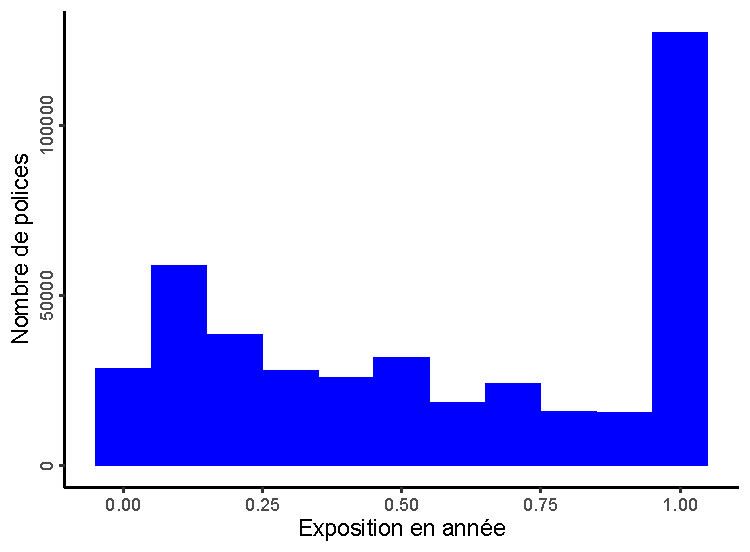
\includegraphics[scale=0.5]{Graphiques/RepartExposure}
\end{minipage}
\end{figure}

La \autoref{fig:ExpoTotFreqMoyRegion} montre la somme des expositions des assurés selon leur région de résidence et la fréquence moyenne observée par région. Une grande proportion de l'expérience du portefeuille provient de la région « Centre ». Il n'y a pas de grosse différence entre chaque région pour la fréquence moyenne observée. 


\begin{figure}
\caption{\label{fig:ExpoTotFreqMoyRegion} Exposition totale par région (gauche), fréquence moyenne observée par région (droite).}
\centering
\begin{minipage}{0.4\linewidth}
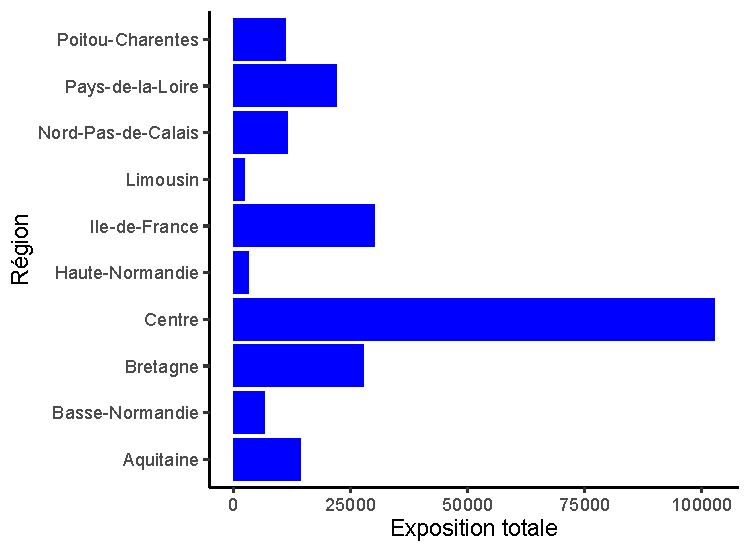
\includegraphics[scale=0.5]{Graphiques/ExpoTotRegion}
\end{minipage}
\hfill
\begin{minipage}{0.4\linewidth}
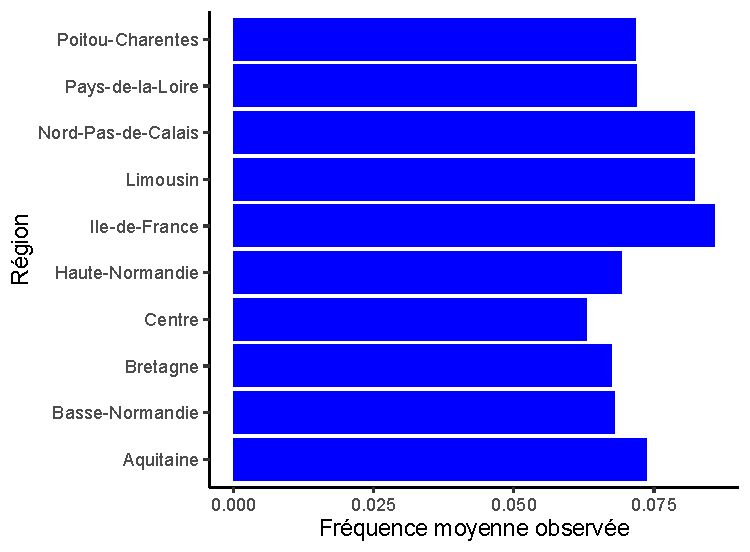
\includegraphics[scale=0.5]{Graphiques/FreqMoyRegion}
\end{minipage}
\end{figure}

La \autoref{fig:ExpoTotFreqMoyPower} montre la répartition de l'expérience en fonction de la catégorie du véhicule et leur fréquence moyenne observée. On voit une augmentation linéaire de la fréquence moyenne en fonction de la puissance du véhicule.

\begin{figure}
\caption{\label{fig:ExpoTotFreqMoyPower} Exposition totale par catégorie de véhicules (gauche), fréquence moyenne observée par catégorie de véhicule (droite).}
\begin{minipage}{0.4\linewidth}
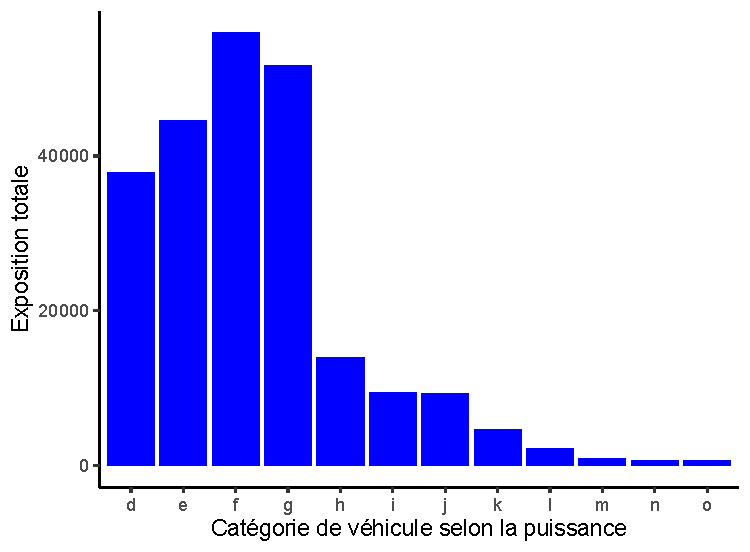
\includegraphics[scale=0.5]{Graphiques/ExpoTotPower}
\end{minipage}
\hfill
\begin{minipage}{0.4\linewidth}
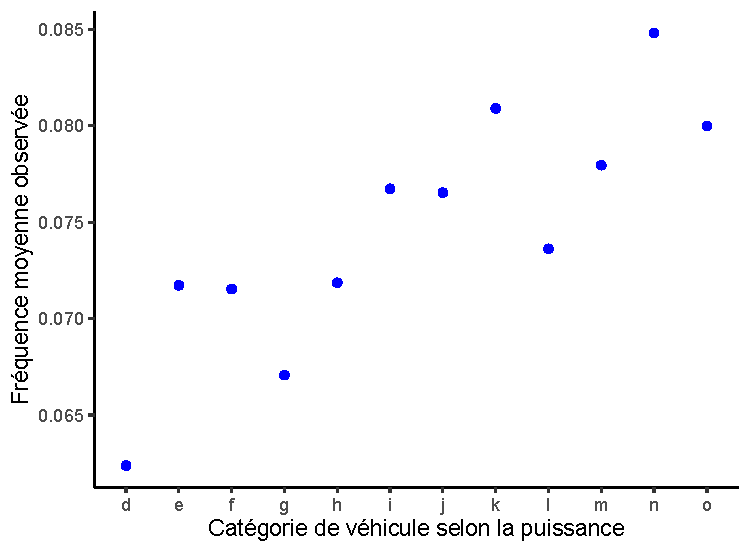
\includegraphics[scale=0.5]{Graphiques/FreqMoyPower}
\end{minipage}
\end{figure}

On observe à la \autoref{fig:ExpoTotFreqMoyCarAge} (droite) une légère augmentation de la fréquence moyenne observée pour l'âge du véhicule allant de 0 à environ 10. Par la suite, la fréquence diminue considérablement. À noter que les véhicules de 20 ans et plus ont été 
groupés. Ces véhicules représentent 8370 observations pour 2,026\% de la base de données.

\begin{figure}
\caption{\label{fig:ExpoTotFreqMoyCarAge} Exposition totale par âge du véhicule avec regroupement des véhicules de plus de 20 ans (gauche), fréquence moyenne observée par âge du véhicule (droite).}
\begin{minipage}{0.4\linewidth}
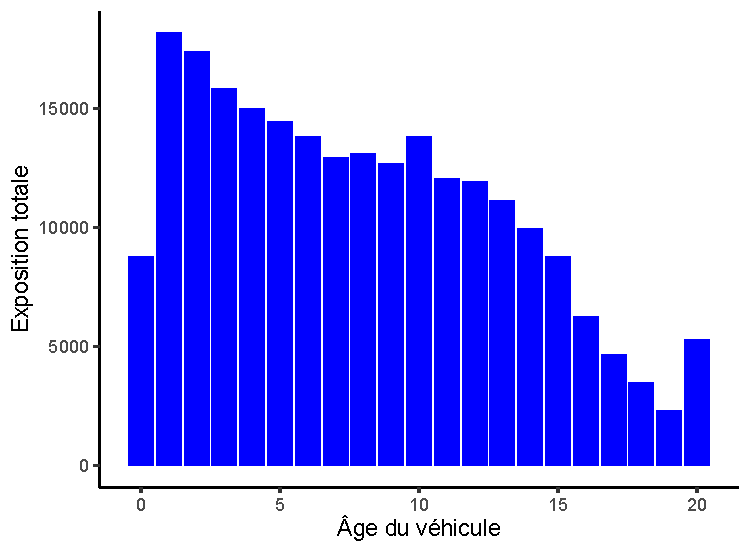
\includegraphics[scale=0.5]{Graphiques/ExpoTotCarAge}
\end{minipage}
\hfill
\begin{minipage}{0.4\linewidth}
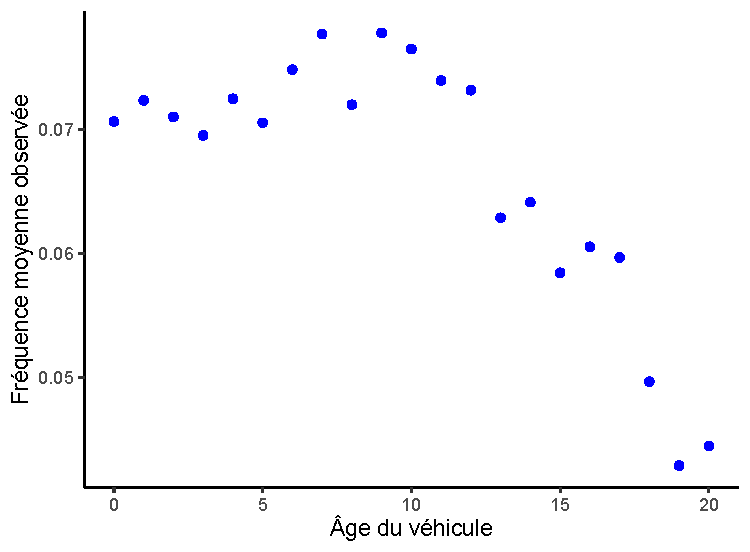
\includegraphics[scale=0.5]{Graphiques/FreqMoyCarAge}
\end{minipage}
\end{figure}

On remarque à la \autoref{fig:ExpoTotFreqMoyDriverAge} un mode autour de 50 ans. On remarque également que les assurés en bas de 25 ans font plus de réclamations. Il y a une légère augmentation de la fréquence moyenne autour de 45 ans. On voit également une variabilité de la fréquence observée pour les âges élevés. Cela est lié au fait qu'il y a peu d'observations (429) pour ces âges. Ainsi, on les regroupe en une catégorie 85 ans et plus.

\begin{figure}
\caption{\label{fig:ExpoTotFreqMoyDriverAge} Exposition totale par âge de l'assuré (gauche), fréquence moyenne observée par âge de l'assuré (droite).}
\begin{minipage}{0.4\linewidth}
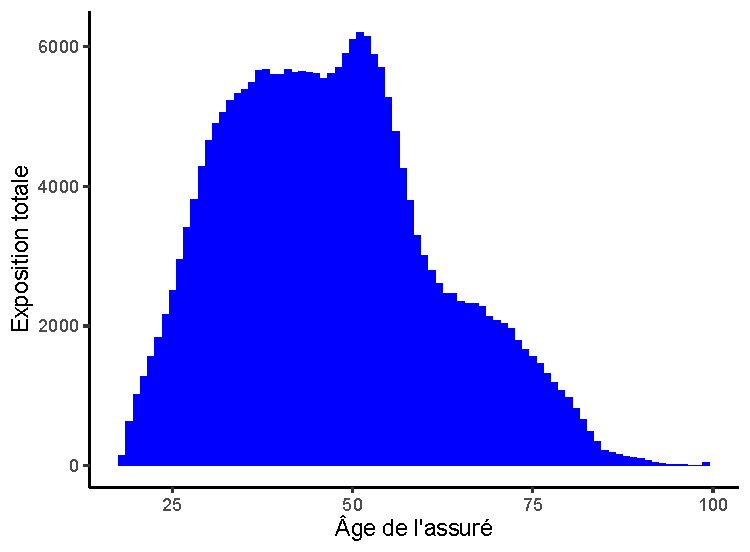
\includegraphics[scale=0.5]{Graphiques/ExpoTotDriverAge}
\end{minipage}
\hfill
\begin{minipage}{0.4\linewidth}
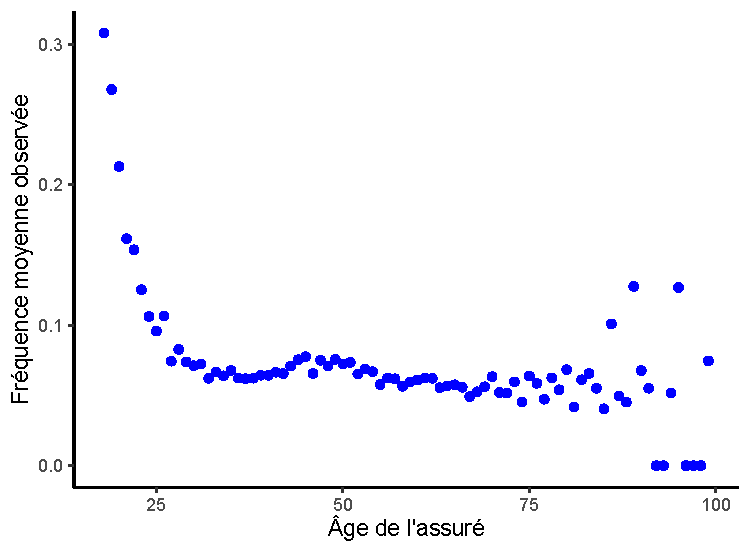
\includegraphics[scale=0.5]{Graphiques/FreqMoyDriverAge}
\end{minipage}
\end{figure}

\begin{figure}
\caption{\label{fig:ExpoTotFreqMoyBrand} Exposition totale par marque de véhicule (gauche), fréquence moyenne observée par marque de véhicule (droite).}
\begin{minipage}{0.4\linewidth}
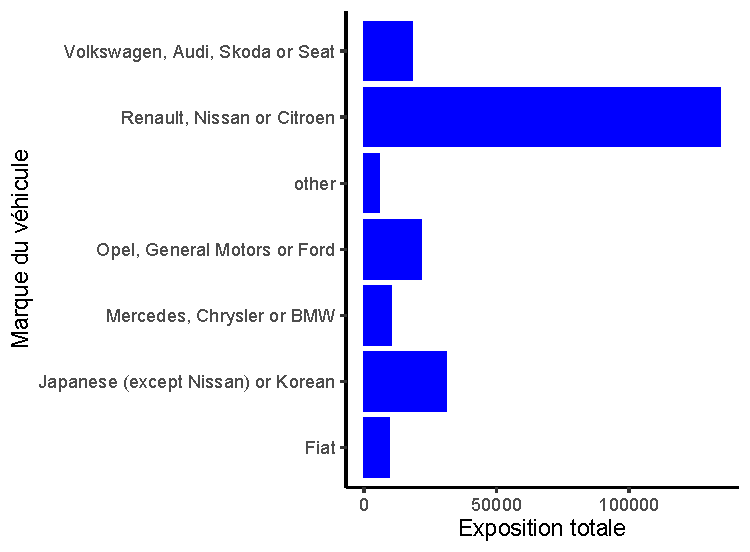
\includegraphics[scale=0.5]{Graphiques/ExpoTotBrand}
\end{minipage}
\hfill
\begin{minipage}{0.4\linewidth}
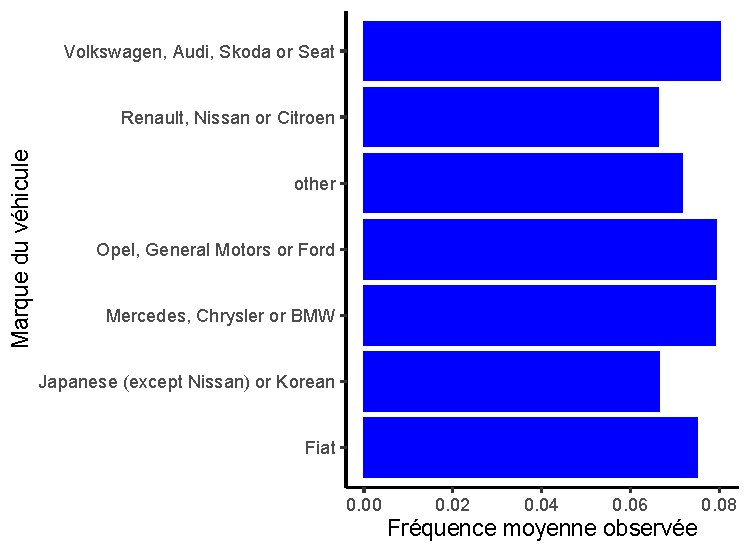
\includegraphics[scale=0.5]{Graphiques/FreqMoyBrand}
\end{minipage}
\end{figure}

\begin{figure}
\caption{\label{fig:ExpoTotFreqMoyGas} Exposition totale par type de carburant (gauche), fréquence moyenne observée par type de carburant (droite).}
\begin{minipage}{0.4\linewidth}
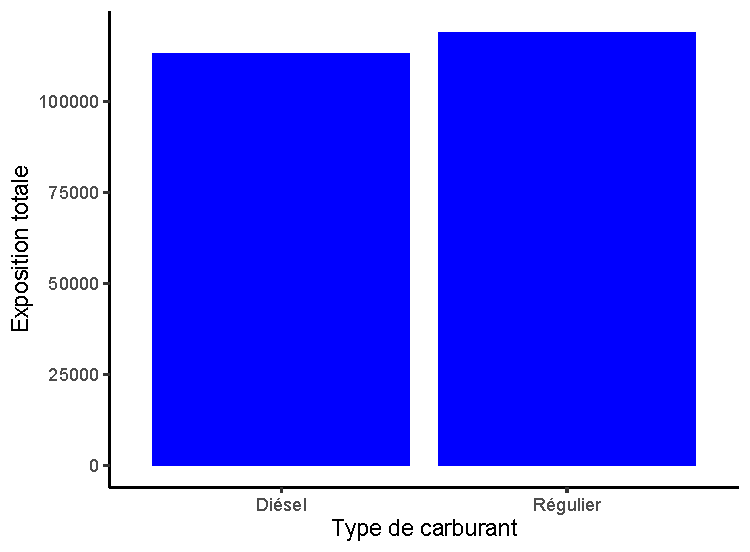
\includegraphics[scale=0.5]{Graphiques/ExpoTotGas}
\end{minipage}
\hfill
\begin{minipage}{0.4\linewidth}
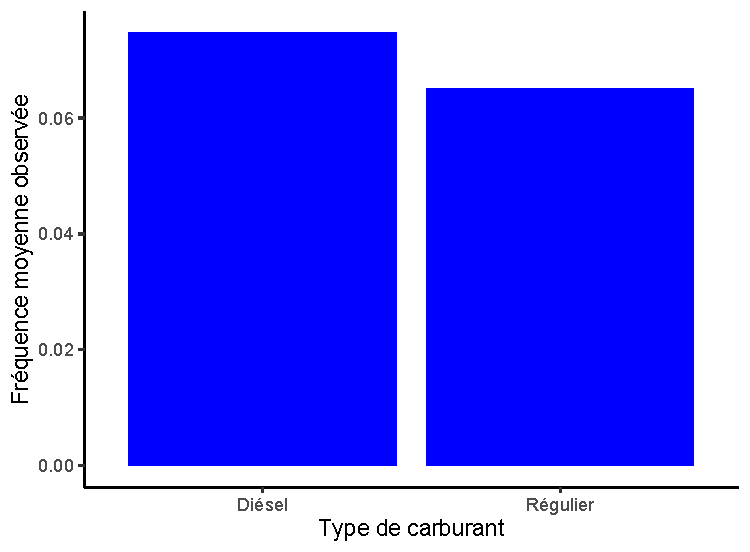
\includegraphics[scale=0.5]{Graphiques/FreqMoyGas}
\end{minipage}
\end{figure}




\section{Modèle de fréquence}
\label{sec:app:modele}

Pour chaque assuré $i$, on a un vecteur de sept dimensions qui représente la $i$\ieme observation:
\begin{align*}
x_i = \left( \text{Power}_i, \text{CarAge}_i, \text{DriverAge}_i, \text{Brand}_i, \text{Gas}_i,
 \text{Region}_i, \text{Density}_i \right)^\prime,\quad i = 1,\dots, 413169.
\end{align*}

On veut prédire $N_i= \verb=ClaimNb=_i \geq 0$ en tenant compte de l'exposition au risque, $v_i = \verb=Exposure=_i $, qui est différente d'un assuré à l'autre. On suppose que chaque observation est indépendante. On a que
\begin{align*}
N_i \sim Poisson\left(\lambda(x_i)v_i\right)
\end{align*}

On sépare les données en trois échantillons disjoints et en stratifiant sur la variable \verb=ClaimNb=. On utilise 60\% des données pour l'échantillon d'entrainement, $\mathcal{D}$, et 20\%  pour l'échantillon de test, $\mathcal{T}$, et l'échantillon de validation, $\mathcal{V}$. Au \autoref{tab:EchanClaimNb}, on voit que la proportion du nombre de réclamation est donc similaire entre chaque échantillon.

\begin{table}[b]
\centering
\caption{\label{tab:EchanClaimNb} Répartition du nombre de réclamations par échantillon}
\begin{tabular}{lrrrrr}
\toprule
 & \multicolumn{5}{c}{ \Verb=ClaimNb= (\%)}\\
\cmidrule{2-6}
Échantillon & 0 & 1 & 2 & 3 & 4\\
\midrule
Entrainement & 96.2751 & 3.5417 & 0.1759 & 0.0065 & 0.0008\\
Test & 96.2740 & 3.5421 & 0.1755 & 0.0073 & 0.0012\\
Validation & 96.2763 & 3.5410 & 0.1755 & 0.0073 & 0.0000\\
\bottomrule
\end{tabular}
\end{table}

On utilise la déviance de Poisson comme fonction de perte:
\begin{align*}
\mathcal{L}(\mathcal{D}, \lambda)=\frac{1}{n} \sum_{i=1}^{n} 2 N_{i}\left[\frac{\lambda\left(\boldsymbol{x}_{i}\right) v_{i}}{N_{i}}-1-\log \left(\frac{\lambda\left(\boldsymbol{x}_{i}\right) v_{i}}{N_{i}}\right)\right].
\end{align*} 

\section{Modèle de base}
\label{sec:modèledebase}

On construit un modèle de base pour pouvoir comparer les réseaux avec celui-ci. On considère un modèle linéaire généralisé Poisson avec le lien logarithmique. On suppose la relation suivante:
\begin{align*}
E\left[ \dfrac{N_i}{v_i} \right] = \exp\left\{ \mathbf{x_i} \boldsymbol\omega\right\}.
\end{align*}
 

On ajuste les données $\mathcal{D}$ à ce modèle. Pour le modèle de base, on considère seulement les effets principaux des variables explicatives. On ajuste le premier modèle suivant:
\begin{align*}
\log\left(\dfrac{\lambda_i}{v_i}\right) = b+ \omega_1 \text{\Verb=DriverAge=}_i + \omega_2 \text{\Verb=Power=}_i + \omega_3 \text{\Verb=CarAge=}_i + \omega_4 \text{\Verb=Region=}_i + \omega_5 \text{\Verb=Gas=}_i + \omega_6 \log\left\{\text{\Verb=Density=}_i\right\}.
\end{align*}

Pour la sélection de variable, on calcule la statistique de Wald pour chaque paramètre estimé. On observe les résultats au \autoref{tab:StatWaldglm1} obtenus à partir de la fonction \textbf{R}, \verb=summary=. La variable \verb=Region= ne semble pas être significative avec  deux niveaux qui obtiennent un seuil observé sous 5\% et seulement un niveau avec un seuil sous 1\%. On vérifie la pertinence de cette variable avec un test de vraisemblance et on retire la variable \verb=Region=. 

\begin{table}
\centering
\caption{\label{tab:StatWaldglm1} Seuil observé de la statistique de Wald pour les paramètres de glm1}
\begin{tabular}{lr}
\toprule
Variable & seuil observé\\
\midrule
(Intercept) & 0.0000000\\
Power & 0.0000025\\
CarAge & 0.0000001\\
DriverAge & 0.0000000\\
\addlinespace
Br.1 & 0.0000000\\
Br.2 & 0.6457504\\
Br.3 & 0.4977571\\
Br.4 & 0.1940670\\
Br.5 & 0.1329266\\
Br.6 & 0.6915220\\
\addlinespace
GasRegular & 0.0000000\\
Re.1 & 0.2459378\\
Re.2 & 0.0065408\\
Re.3 & 0.0560250\\
Re.4 & 0.6325997\\
\addlinespace
Re.5 & 0.1563482\\
Re.6 & 0.0264359\\
Re.7 & 0.5915649\\
Re.8 & 0.0579710\\
Re.9 & 0.5396968\\
\addlinespace
Density & 0.0000000\\
\bottomrule
\end{tabular}
\end{table}


\begin{table}
\centering
\caption{\label{tab:LRTglm1} Résultats des test du ratio de vraisemblance pour glm1}
\begin{tabular}{lrrr}
\toprule
  & Df & LRT & Pr(>Chi)\\
\midrule
Power & 1 & 21.83182 & 0.0000030\\
CarAge & 1 & 28.25304 & 0.0000001\\
DriverAge & 1 & 211.92967 & 0.0000000\\
Brand & 6 & 86.29772 & 0.0000000\\
Gas & 1 & 35.54875 & 0.0000000\\
\addlinespace
Region & 9 & 19.25317 & 0.0231243\\
$\log\{Density\}$ & 1 & 261.57895 & 0.0000000\\
\bottomrule
\end{tabular}
\end{table}



\section{Pré-traitement des données pour les réseaux de neurones}
\label{sec:app:pretraitement}

On doit traiter les variables avant d'entrainer les réseaux de neurones. Ceux-ci peuvent traiter seulement des variables numériques, ainsi on doit transformer les variables catégorielles. Les variables continues doivent, quant à elles, être standardisées. Cela permet d'avoir une performance plus rapide. %ajouter une source

\subsection{Traitement des variables catégorielles}

La variable \verb=Power= est transformée en facteur de 1 à 12. La variable \verb=Gas= est transformée en variable binaire, où \Verb@Regular@ $=1$ et \Verb@Diesel@ $=0$. Pour les variables \verb=Region= et \verb=Brand=, on utilise deux façons de les traiter et on compare leurs résultats dans l'analyse. La première façon est de créer ($k-1$) variables binaires pour une variable catégorielle avec $k$ niveaux. 

La deuxième méthode qu'on utilise est une technique d'apprentissage de la représentation ( « representation learning » ). Il s'agit d'ajouter des couches de plongement ( « embedding layers» ) au réseau qui permettent de réduire la dimension de ces variables catégorielles, voir \citet{richman2018ai}.


En appliquant la première méthode, on obtient un vecteur de variables explicatives de 20 dimensions
\begin{align*}
\mathcal{X} \subset[1,12] \times\{0,1\} \times\{0,1\}^{7} \times\{0,1\}^{9} \times[0,100] \times[0,90] \times[2,27000].
\end{align*}

La deuxième méthode permet de réduire la dimension de \verb=Region= et \verb=Brand= à $d=2$ et ainsi on obtient un vecteur de variables explicatives de 9 dimensions. 





\subsection{Traitement des variables continues}
\label{subsec:TraitementVarContinues}

Premièrement, on applique la transformation $log$ à la variable \verb=Density=. Par la suite, on doit s'assurer que chaque variable soit sur la même échelle. On utilise la transformation suivante pour les variables \verb=DriverAge=, \verb=CarAge=, \verb=Power= et \verb=log(Density)=:
\begin{align*}
\frac{x_i-\min (x_i)}{\max (x_i)-\min (x_i)} \mapsto [0,1].
\end{align*}

\section{Réseaux utilisés}
\label{sec:app:reseauxutilisés}

On détaille dans cette section la démarche utilisée pour construire les différents modèles. 

Tout d'abord, on fera une distinction entre les réseaux à une seule couche cachée et ceux à plusieurs couches cachées. Selon %source
, les réseaux de neurones à une seule couche sont capables d'approximer n'importe quelle fonction non linéaire. On verra toutefois que le fait d'ajouter des couches cachées au réseau permet d'apprendre les interactions entre les variables explicatives plus efficacement. Ensuite, on compare la différence entre les réseaux utilisant l'approche des variables binaires et les réseaux utilisant l'approche des couches de plongement. %Finalement on parle de la méthode Cann

On utilise le paquetage \verb=keras= qui est une interface au logiciel du même nom, \citep{keras}.
Comme mentionné à la section 4 de \citet{ferrario2018insights}, on est pas intéressé à trouver le minimum total de $\mathcal{L}(\mathcal{D}, \hat{\lambda})$ étant donné de la sur-paramétrisation des réseaux. L'idée est d'arrêter au bon moment l'algorithme de rétro-propagation. On y arrive en établissant une règle d'arrêt qui sera la même pour tous les réseaux ajustés. On arrête l'entrainement lorsque l'erreur de validation ne s'est pas améliorée depuis 20 epochs et on demande au modèle de retourner les paramètres qui permettent d'obtenir la plus petite erreur de validation. De cette façon, on s'assure de ne pas surajuster le modèle. Le \autoref{code:regleArret} montre comment on implémente cela avec \verb=keras=. De plus, pour chaque réseau on utilise, évidemment, le même échantillon de validation $\mathcal{V}$. On fixe la taille de mini-lot ( « mini-batch » ) à 8192. On établit un taux de réduction du taux d'apprentissage de 0.05. Ainsi, lorsque l'erreur de validation ne s'est pas améliorée depuis 10 epochs, on obtient un taux d'apprentissage 20 fois plus petit que le précédant. Cela permet à l'algorithme de tenter de quitter des points de selle, où le gradient de la fonction de perte est nul ou presque.% ajouter une référence


\begin{lstlisting}[caption= {Définition des paramètres de l'algorithme},label=code:regleArret]
	model %>% fit(list(XlearnNN, WlearnNN), 
              	YlearnNN,
              	validation_data = list(list(XvalNN,WvalNN),YvalNN),
              	epochs = 1000, 
              	batch_size = 8192,
              	callbacks = list(callback_early_stopping(patience = 20, 
              			restore_best_weights = T),
              	callback_reduce_lr_on_plateau(factor = 0.05)
              	)
              	)
\end{lstlisting}



\subsection{Réseau de neurones « shallow »}
\label{subsec:Shallow}

Comme mentionné précédemment, on ne cherche pas à trouver \emph{le} meilleur modèle, mais bien \emph{un} des meilleurs modèles. Ainsi, la méthode utilisée pour trouver les hyperparamètres du modèle final vise à améliorer une structure de base avec certains hyperparamètres. Cette structure de base se traduit par le nombre de neurones dans la couche cachée que l'on fixe. Le \autoref{tab:resultsShallow} montre l'erreur de validation pour $q_1 \in \left\{8, 16, 32, 64, 128 ,256 ,512\right\}$ avec la règle d'arrêt mentionnée antérieurement. On fixe donc le nombre de neurones à 32 et on tente d'optimiser le taux d'abandon, $d$, et les taux de régularisation, $\ell_2$ et $\ell_2$, à l'aide d'une grille de recherche disponible au \autoref{tab:rechercheShallow} de l'\autoref{ann:grilleRecherche}.

\begin{table}
\centering
\caption{\label{tab:resultsShallow} Résultats de la recherche du nombre de neurones pour le réseau avec une couche cachée}
\begin{tabularx}{0.6\textwidth}{Xrrr}
\toprule
Nombre \newline de neurones & $\mathcal{L}\left\{\mathcal{V},\hat{\lambda} \right\} $ & $\mathcal{L}\left\{\mathcal{D},\hat{\lambda} \right\} $ &  Epochs\\
\midrule
32 & \textbf{0.2511} & 0.2503 & 51\\
64 & 0.2516 & 0.2512 & 58\\
16 & 0.2518 & 0.2523 & 45\\
512 & 0.2519 & 0.2490 & 33\\
256 & 0.2519 & 0.2496 & 37\\
\addlinespace
128 & 0.2520 & 0.2510 & 33\\
8 & 0.2521 & 0.2523 & 100\\
\bottomrule
\end{tabularx}
\end{table}


On présente les six meilleurs résultats dans le \autoref{tab:resultsShallow32}. Le réseau qui offre la plus petite erreur de validation est celui avec $d=0.25$. On remarque qu'aucun des trois meilleurs modèles n'inclut une régularisation $\ell_1$ ou $\ell_2$. Une grille de recherche plus grande aurait peut-être permis de diminuer l'erreur à l'aide d'autres valeurs pour les taux de régularisation. On se limite à ces valeurs par souci de temps. Toutefois, on verra à l'aide des autres modèles que le taux d'abandon offre de meilleurs résultats , et ce  plus efficacement que les taux de régularisation.


\begin{table}
\centering
\caption[Résultats du réseau d'une couche cachée avec 32 neurones]{\label{tab:resultsShallow32} Résultats de la recherche des hyperparamètres pour le réseau de neurone d'une couche cachée avec 32 neurones}
\begin{tabular}{rrrrrr}
\toprule
$\mathcal{L}\left\{\mathcal{V},\hat{\lambda} \right\} $ & $\mathcal{L}\left\{\mathcal{D},\hat{\lambda} \right\} $ & $d$ & $\ell_1$ & $\ell_2$ & Epochs\\
\midrule
\textbf{0.2508} & 0.2512 & 0.25 & 0 & 0 & 66\\
0.2510 & 0.2518 & 0.50 & 0 & 0 & 70\\
0.2510 & 0.2504 & 0.00 & 0 & 0 & 54\\
0.2511 & 0.2519 & 0.50 & 0 & 0.001 & 79\\
0.2513 & 0.2520 & 0.25 & 0.001 & 0.001 & 82\\
0.2514 & 0.2526 & 0.50 & 0.001 & 0.001 & 125\\
\bottomrule
\end{tabular}
\end{table}

\subsection{Réseau à deux couches cachées}
\label{subsec:deep2}

On utilise la même méthode que pour le réseau à une couche cachée. On tente de fixer le nombre de neurones par couche en premier. On cherche parmi une combinaison de $q_1 \in \left\{ 8, 16, 32, 64 \right\}$, et $q_2\in \left\{8,16,32,64 \right\}$. On obtient les résultats au \autoref{tab:ResultsDeep2}. La combinaison $(q_1,q_2) = (8,8)$ donne la plus petite erreur de validation. Cependant, on tente également d'optimiser le modèle avec $(q_1,q_2)=(32,16)$. L'erreur d'entrainement pour cette combinaison est largement inférieure à $(q_1,q_2) = (8,8)$ et le nombre d'epochs est plus bas. Il est probable que le nombre plus élevé de paramètres fasse en sorte qu'il surajuste rapidement les données d'entrainement et, ainsi, l'algorithme exerce la règle d'arrêt rapidement. On peut donc penser que ce réseau pourrait bénéficier d'une régularisation quelconque. Ainsi, on fait une grille de recherche pour les deux réseaux mentionnés des hyperparamètres $d_1$, $d_2$, $\ell_1$ et $\ell_2$. Les valeurs de la grille sont au \autoref{tab:rechercheDeep2} de l'\autoref{ann:grilleRecherche}. On utilise les mêmes taux de régularisation sur les deux couches cachées, mais on utilise deux taux d'abandon différents.  Le \autoref{code:deep2} montre aux lignes  3 et 7 qu'on utilise \verb=FLAGS$l1= et \verb=FLAGS$l2= à chaque couche. On utilise également des couches de normalisation, aux lignes 4 et 8, qui permettent de standardiser la sortie de chaque neurone de la couche précédente. Cela permet d'éviter le problème de gradient disparaissant.%ajouter source


\begin{table}
\centering
\caption{\label{tab:ResultsDeep2} Résultats de la recherche du nombre de neurones par couche pour le réseau avec deux couches cachées}
\begin{tabularx}{0.6\textwidth}{Xrrr}
\toprule
Nombre \newline de neurones & $\mathcal{L}\left\{\mathcal{V},\hat{\lambda} \right\} $ & $\mathcal{L}\left\{\mathcal{D},\hat{\lambda} \right\} $ & Epochs\\
\midrule
(8, 8) & \textbf{0.2512} & 0.2510 & 64\\
(32, 16) & \textbf{0.2514} & 0.2496 & 46\\
(16, 32) & 0.2514 & 0.2504 & 55\\
(16, 16) & 0.2516 & 0.2505 & 54\\
(16, 64) & 0.2517 & 0.2502 & 49\\
(32, 32) & 0.2517 & 0.2498 & 44\\
\bottomrule
\end{tabularx}
\end{table}

\begin{lstlisting}[caption = {Définition de la structure du réseau à deux couches cachées}, label= code:deep2]
 net <- features.0 %>%
  layer_dense(units = FLAGS$hidden1,activation="relu",kernel_initializer = initializer_he_normal(seed=2L),
              kernel_regularizer = regularizer_l1_l2(l1 = FLAGS$l1, l2 = FLAGS$l2)) %>% 
  layer_batch_normalization() %>%
  layer_dropout(rate=FLAGS$dropout1) %>% 
  layer_dense(units = FLAGS$hidden2,activation="relu",kernel_initializer = initializer_he_normal(seed=3L),
              kernel_regularizer = regularizer_l1_l2(l1 = FLAGS$l1, l2 = FLAGS$l2)) %>% 
  layer_batch_normalization() %>%
  layer_dropout(rate=FLAGS$dropout2) %>% 
  layer_dense(units=1, activation='linear', 
              weights=list(array(0, dim=c(FLAGS$hidden2,1)), 
              	array(log(lambda.hom), dim=c(1))))
\end{lstlisting}


On présente les six meilleurs réseaux au \autoref{tab:ResultsDeep2Tuning}.  On sélectionne le modèle avec 32 et 16 neurones et $d_2=0.25$. Encore une fois, on remarque qu'aucun des meilleurs modèles ne contient une régularisation $\ell_1$ ou $\ell_2$.

\begin{table}
\centering
\caption{\label{tab:ResultsDeep2Tuning}Résultats de la recherche des hyperparamètres pour les réseaux à deux couches cachées}
\begin{tabularx}{0.8\textwidth}{Xrrrrrrr}
\toprule
Nombre \newline de neurones & $\mathcal{L}\left\{\mathcal{V},\hat{\lambda} \right\} $ & $\mathcal{L}\left\{\mathcal{D},\hat{\lambda} \right\} $ & $d_1$ & $d_2$ & $\ell_1$ & $\ell_2$ & Epochs\\
\midrule
(32, 16) & \textbf{0.2510} & 0.2504 & 0.00 & 0.25 & 0 & 0 & 56\\
(32, 16) & 0.2510 & 0.2511 & 0.25 & 0.25 & 0 & 0 & 72\\
(8, 8) & 0.2511 & 0.2515 & 0.00 & 0.25 & 0 & 0 & 76\\
(32, 16) & 0.2511 & 0.2503 & 0.00 & 0.25 & 0 & 0 & 57\\
(32, 16) & 0.2511 & 0.2511 & 0.25 & 0.00 & 0 & 0 & 111\\
(8, 8) & 0.2512 & 0.2524 & 0.00 & 0.50 & 0 & 0 & 80\\
\bottomrule
\end{tabularx}
\end{table}

\subsection{Réseau à trois couches cachées}
\label{subsec:Deep3}

Pour le réseau à trois couches cachées, on teste d'abord le nombre de neurones par couche avec la combinaison des paramètres suivants: $q_1\in \left\{8, 16, 32 \right\}$, $q_2 \in \left\{8, 16, 32 \right\}$ et $q_3\in \left\{8, 16, 32 \right\}$. Un total de 27 possibilités sont testées. On présente les six meilleurs résultats au \autoref{tab:ResultsDeep3}. Pour les mêmes raisons énumérées à la \autoref{subsec:deep2}, on tente d'optimiser les hyperparamètres des modèles $(q_1,q_2,q_3) = (8,8,8)$ et $(q_1,q_2,q_3) = (32,16,8)$. 
Par souci de temps, on tente d'optimiser d'abord $d_1$ et $d_2$ pour ensuite tenter d'ajouter une régularisation $\ell_1$ ou $\ell_2$. À noter qu'on n'ajoute pas de taux d'abandon à la troisième couche cachée pour économiser le temps de calcul. On utilise la grille de recherche au \autoref{tab:rechercheDeep3} de l'\autoref{ann:grilleRecherche}. 

\begin{table}[b]
\centering
\caption{\label{tab:ResultsDeep3} Résultats de la recherche du nombre de neurones par couche pour le réseau avec trois couches cachées}
\begin{tabularx}{0.6\textwidth}{Xrrr}
\toprule
Nombre \newline de neurones & $\mathcal{L}\left\{\mathcal{V},\hat{\lambda} \right\} $ & $\mathcal{L}\left\{\mathcal{D},\hat{\lambda} \right\} $ & Epochs\\
\midrule
(8, 8, 8) & \textbf{0.2513} & 0.2507 & 72\\
(8, 8, 16) & 0.2519 & 0.2508 & 63\\
(32, 8, 8) & 0.2520 & 0.2501 & 35\\
(16, 8, 8) & 0.2520 & 0.2500 & 49\\
(32, 8, 16) & 0.2521 & 0.2500 & 46\\
\addlinespace
(32, 16, 8) & \textbf{0.2521} & \textbf{0.2492} & 37\\
\bottomrule
\end{tabularx}
\end{table}

Les résultats du \autoref{tab:ResultsDeep3Tuning} montrent que le réseau $(q_1,q_2,q_3)=(32,16,8)$ avec un taux d'abandon $d_2=0.5$ obtient la plus petite erreur de validation. 

\begin{table}
\centering
\caption{\label{tab:ResultsDeep3Tuning}Résultats de la recherche des hyperparamètres pour le réseau à trois couches cachées}
\begin{tabularx}{0.8\textwidth}{Xrrrrrrr}
\toprule
Nombre \newline de neurones & $\mathcal{L}\left\{\mathcal{V},\hat{\lambda} \right\} $ & $\mathcal{L}\left\{\mathcal{D},\hat{\lambda} \right\} $ & $d_1$ & $d_2$ & $\ell_1$ & $\ell_2$ & Epochs\\
\midrule
(32, 16, 8) & 0.2510 & 0.2511 & 0.00 & 0.50 & 0 & 0 & 72\\
(8, 8, 8) & 0.2511 & 0.2523 & 0.25 & 0.25 & 0 & 0 & 59\\
(8, 8, 8) & 0.2512 & 0.2514 & 0.00 & 0.25 & 0 & 0 & 83\\
(32, 16, 8) & 0.2512 & 0.2513 & 0.25 & 0.00 & 0 & 0 & 54\\
(8, 8, 8) & 0.2513 & 0.2517 & 0.25 & 0.00 & 0 & 0 & 59\\
\addlinespace
(32, 16, 8) & 0.2515 & 0.2528 & 0.50 & 0.25 & 0 & 0 & 71\\
\bottomrule
\end{tabularx}
\end{table}

\subsection{Réseau à quatre couches cachées}
\label{subsec:deep4}

Comme à la \autoref{subsec:Deep3}, on cherche d'abord quelle combinaison de neurones par couches cachées permet d'obtenir la plus petite erreur de validation parmi $q_1 \in \left\{8, 16, 32 \right\}$, $q_2 \in \left\{8, 16, 32 \right\}$, $q_3 \in \left\{8, 16\right\}$ et $q_4 \in \left\{8, 16 \right\}$. On fait ensuite une grille de recherche pour les hyperparamètres $d_1$, $d_2$ et $d_3$. Finalement, on optimise les hyperparamètres $\ell_1$ et $\ell_2$ par une autre grille de recherche, voir \autoref{tab:rechercheDeep4}. 

\begin{table}
\centering
\caption{\label{tab:ResultsDeep4} Résultats de la recherche du nombre de neurones par couche pour le réseau avec quatre couches cachées}
\begin{tabularx}{0.6\textwidth}{Xrrr}
\toprule
Nombre \newline de neurones & $\mathcal{L}\left\{\mathcal{V},\hat{\lambda} \right\} $ & $\mathcal{L}\left\{\mathcal{D},\hat{\lambda} \right\} $ & Epochs\\
\midrule
(16,16,16,16) & 0.2523 & 0.2501 & 34\\
(16,16,16,8) & 0.2524 & 0.2502 & 37\\
(16,32,16,16) & 0.2525 & 0.2494 & 35\\
(16,16,8,8) & 0.2525 & 0.2509 & 32\\
(16,32,8,16) & 0.2526 & 0.2489 & 42\\
\addlinespace
(16,8,16,8) & 0.2526 & 0.2513 & 42\\
\bottomrule
\end{tabularx}
\end{table}

\begin{table}
\centering
\caption{\label{tab:ResultsDeep4Tuning}Résultats de la recherche des hyperparamètres pour le réseau à quatre couches cachées}
\begin{tabularx}{0.9\textwidth}{Xrrrrrrrr}
\toprule
Nombre \newline de neurones & $\mathcal{L}\left\{\mathcal{V},\hat{\lambda} \right\} $ & $\mathcal{L}\left\{\mathcal{D},\hat{\lambda} \right\} $ & $d_1$ & $d_2$ & $d_3$ & $\ell_1$ & $\ell_2$ & Epochs\\
\midrule
(16,32,8,16) & 0.2514 & 0.2511 & 0.0 & 0.0 & 0.5 & 0e+00 & 0 & 133\\
(16,32,8,16) & 0.2515 & 0.2507 & 0.0 & 0.0 & 0.5 & 0e+00 & 0 & 98\\
(16,16,16,16) & 0.2517 & 0.2529 & 0.5 & 0.0 & 0.0 & 0e+00 & 0 & 67\\
(16,16,16,16) & 0.2517 & 0.2526 & 0.5 & 0.0 & 0.0 & 0e+00 & 0 & 66\\
(16,32,8,16) & 0.2517 & 0.2511 & 0.0 & 0.0 & 0.5 & 1e-06 & 0 & 98\\
\addlinespace
(16,16,16,16) & 0.2518 & 0.2523 & 0.0 & 0.5 & 0.0 & 0e+00 & 0 & 62\\
\bottomrule
\end{tabularx}
\end{table}

\subsection{Réseaux Cann et réseaux avec couches de plongement}
\label{subsec:CannEmbed}

Par souci de temps, les réseaux Cann et les réseaux avec couches de plongement n'ont pas été optimisés au niveau de leurs hyperparamètres. On a utilisé les valeurs trouvées à l'aide des réseaux simples. On optimise seulement le nombre d'epochs à l'aide de la même règle d'arrêt. On présente les résultats finaux au \autoref{tab:resultsTOT} classés en ordre de performance. On constate que tous les modèles performent mieux que le modèle de base. Un autre constat est que les couches de plongement améliorent la performance. En effet, tous les six meilleures modèles sont des modèles avec des couches de plongement.  Le seul modèle qui semble s'approcher de la performance est le Shallow, qui arrive à battre les modèles à quatre couches et couches de plongement. Cependant, pour les trois types de modèles, la structure qui performent le moins est celle avec quatre couches. Ainsi, le Shallow bat les modèles à quatres couches par défaut. C'est probablement l'inverse qui se produit, soit qu'une structure à quatre couches est trop complexe pour ce problème.

Une autre importante information qu'on retire de ces résultats est le fait que les modèles Cann sont plus performant que les modèles avec plongement pour chaque structure. L'initialisation par le Glm permet donc d'améliorer  les modèles avec constance.   


\begin{table}
\centering
\caption{\label{tab:resultsTOT} Résultats de l'erreur sur les données de test pour tous les modèles}
\begin{tabular}{lrrrr}
\toprule
Modèle & $\mathcal{L}\left\{\mathcal{T},\hat{\lambda} \right\} $ & $\mathcal{L}\left\{\mathcal{D},\hat{\lambda} \right\} $ & $\mathcal{L}\left\{\mathcal{V},\hat{\lambda} \right\} $ & Epochs\\
\midrule
CannDeep3 & 0.25049 & 0.25086 & 0.25064 & 78\\
Deep3Embedding & 0.25051 & 0.25075 & 0.25046 & 53\\
CannDeep2 & 0.25054 & 0.25018 & 0.25026 & 51\\
Deep2Embedding & 0.25060 & 0.25029 & 0.25026 & 48\\
CannShallow & 0.25061 & 0.25099 & 0.25045 & 102\\
\addlinespace
ShallowEmbedding & 0.25066 & 0.25093 & 0.25044 & 79\\
Shallow & 0.25077 & 0.25103 & 0.25076 & 56\\
CannDeep4 & 0.25097 & 0.25125 & 0.25112 & 99\\
Deep3 & 0.25099 & 0.25074 & 0.25095 & 80\\
Deep4Embedding & 0.25101& 0.25141 & 0.25084 & 82\\
\addlinespace
Deep2 & 0.25102 & 0.25018 & 0.25113 & 70\\
Deep4 & 0.25152 & 0.25044 & 0.25140 & 66\\
Glm	  & 0.25175 & 0.25311 &    -    &  - \\
\bottomrule
\end{tabular}
\end{table}



\section{Comparaison et interprétation des modèles}
\label{sec:ComparaisonInterpretation}

Cette section est basée sur \citet{molnar2019} et le chapitre 16 de \citet{boehmke2019hands}.

On compare dans cette section les modèles Canndeep3, CannShallow et Glm. On vise à comprendre les différences entre le meilleure modèle, le meilleure modèle avec une seule couche et le modèle de base. On utilise les graphiques de dépendance partielle (PDP), les graphiques d'espérance conditionnelle individuelle (ICE) et la statistique H de Friedman ,\citet{friedman2008predictive}, pour trouver les interactions entre les variables explicatives. On applique aussi ces techniques au Glm pour pouvoir identifier ses faiblesses. 

On résume tout d'abord ces trois techniques.

\subsection{Interprétation de la boîte noire}
\label{subsec:BlackBox}

\subsubsection*{Graphique de dépendance partielle}

Les PDPs permettent de visualiser comment une variable explicative influence la prévision du modèle. Soit $x_{\ell},\;\ell \in \{1,\dots, p \}$, la variable explicative d'intérêt, on fixe sa valeur et on calcule la moyenne des prévisions sur les valeurs des autres variables explicatives:
\begin{align*}
\bar{f}_{\ell}\left(x_{\ell}\right)=\frac{1}{n} \sum_{i=1}^{n} f_{\text {model }}\left(x_{\ell}, \boldsymbol{x}_{i}^{(-\ell)}\right).
\end{align*}

Le vecteur $\boldsymbol{x}_{i}^{(-\ell)}$ contient toutes les valeurs observées des variables explicatives pour $i$ sauf la variable $x_{\ell}$. En calculant cette moyenne pour plusieurs valeurs fixées de $x_{\ell}$ on obtient donc un graphique de la réponse prédite en fonction de la variable d'intérêt. 


\subsubsection*{Graphique d'espérance conditionnelle individuelle}

Les ICEs sont semblables aux PDPs. Leur différence est qu'on ne prend pas la moyenne des observations pour une valeur fixe de la variable d'intérêt. On applique:
\begin{align*}\tilde{f}_{\ell, i}\left(x_{\ell}\right)=f_{\text {model }}\left(x_{\ell}, \boldsymbol{x}_{i}^{(-\ell)}\right).
\end{align*}
On regarde ainsi comment la variable d'intérêt influence la prévision de chaque observation. 

\subsubsection*{Statistique H de Friedman}

La statistique H de Friedman permet de mesurer l'interaction entre deux ou mêmes plusieurs variables explicatives. Elle s'interprète par la part de la variance de la prévision qui est expliquée par l'interaction. On montre l'équation pour l'interaction entre deux variables,$x_k$ et $x_\ell$:
\begin{align*}
H_{k \ell}^{2}=\frac{\sum_{i=1}^{n}\left\{\bar{f}_{k l}\left(x_{i, k}, x_{i, \ell}\right)-\bar{f}_{k}\left(x_{i, k}\right)-\bar{f}_{l}\left(x_{i, \ell}\right)\right\}^{2}}{\sum_{i=1}^{n} \bar{f}_{k l}^{2}\left(x_{i, k}, x_{i, \ell}\right)},
\end{align*}
où $\bar{f}_{k}\left(x_{k}\right)$ et $\bar{f}_{l}\left(x_{\ell}\right)$ sont les PDPs univariés et $\bar{f}_{k l}\left(x_{k}, x_{\ell}\right)$ est le PDP bivarié. Une valeur de $H=0$ signifie aucune interaction, tandis qu'une valeur de $H=1$ signifie que l'effet des variables sur la prévision ne se transmet que par l'interaction de ces deux variables.


\subsection{Analyse et interprétation}
\label{subsec:AnalyseInterpret}


On utilise le paquetage \verb=iml= pour réaliser l'interprétation des modèles, \citep{package:iml}. Tous les graphiques et calculs ont été réalisés avec un sous-ensemble aléatoire de 1000 observations de l'ensemble de la base de donnée.


Tout d'abord, on passe en revue les PDPs univariés les plus intéressants. On continue ensuite avec les ICEs et puis avec le calcul de la statistique H pour les deux réseaux. À l'aide des résultats de cette statistique, on trace les PDPs bivariés les plus interessants. 


La \autoref{fig:pdp3DriverAge} montre une lacune du modèle Glm. L'effet de l'âge selon ce modèle est linéaire. Les deux réseaux captent le même effet de cette variable ou presque. Le modèle CannDeep3 prédit des fréquences plus élevées pour les jeunes conducteurs. 
 
\begin{figure}
\centering
\caption{\label{fig:pdp3DriverAge} Dépendence partielle pour la variable DriverAge pour les trois modèles sélectionnés }
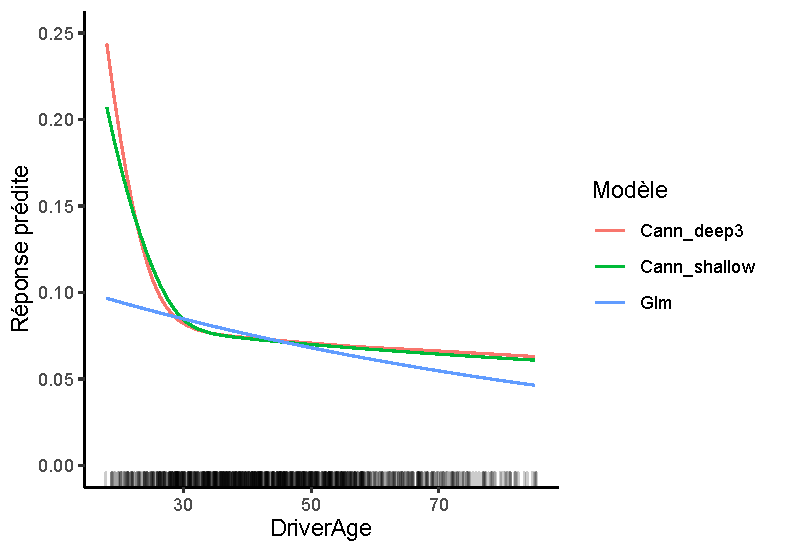
\includegraphics[scale=0.9]{Graphiques/pdp3modDriverAge}
\end{figure}




La \autoref{fig:pdp3CarAge} montre bien une différence entre les deux réseaux. Comme on le constatait à la \autoref{fig:ExpoTotFreqMoyCarAge}, le modèle CannDeep3 fait ressortir une augmentation de la fréquence prédite pour les véhicules âgés de 5 à 10 ans. Les deux autres modèles ne captent pas cet effet.


\begin{figure}
\centering
\caption{\label{fig:pdp3CarAge} Dépendance partielle pour la variable CarAge pour les trois modèles sélectionnés }
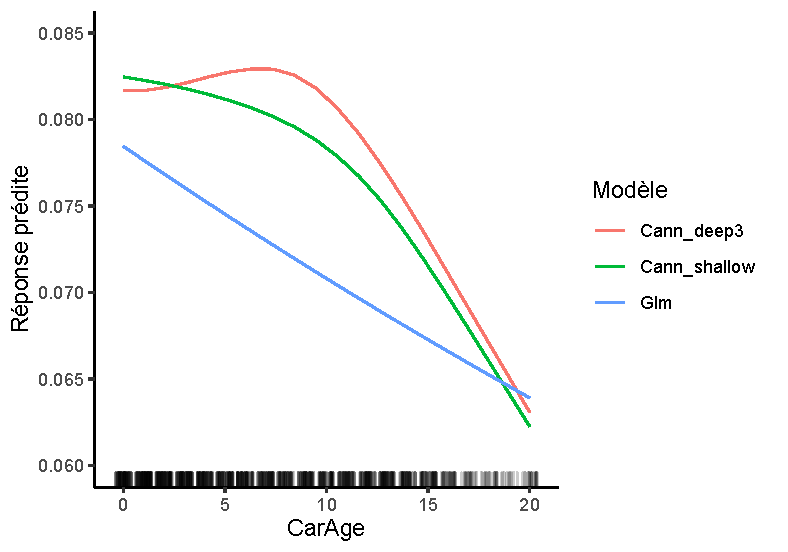
\includegraphics[scale=0.9]{Graphiques/pdpMod3CarAge}
\end{figure}

\begin{figure}
\caption{\label{fig:ice3Car} ICE pour la variable CarAge pour les trois modèles sélectionnés}
\centering
\begin{minipage}{0.45\linewidth}
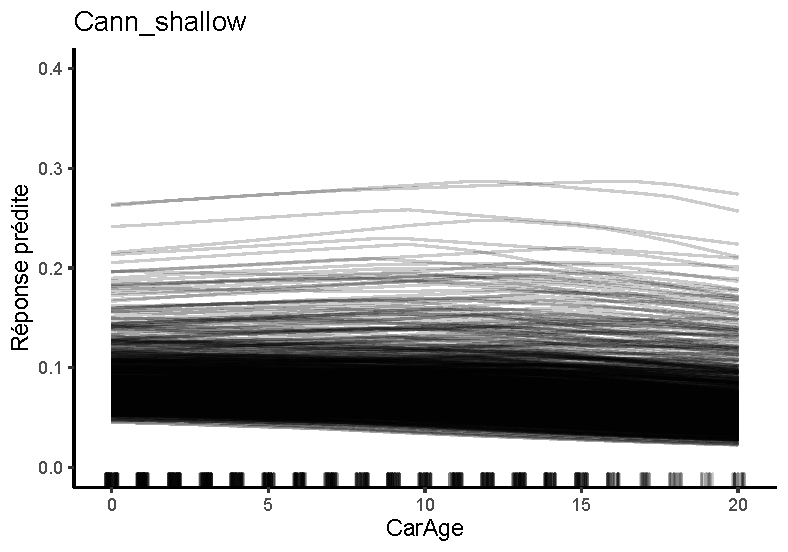
\includegraphics[scale=0.6]{Graphiques/iceCarShallow}
\end{minipage}
\hfill
\begin{minipage}{0.45\linewidth}
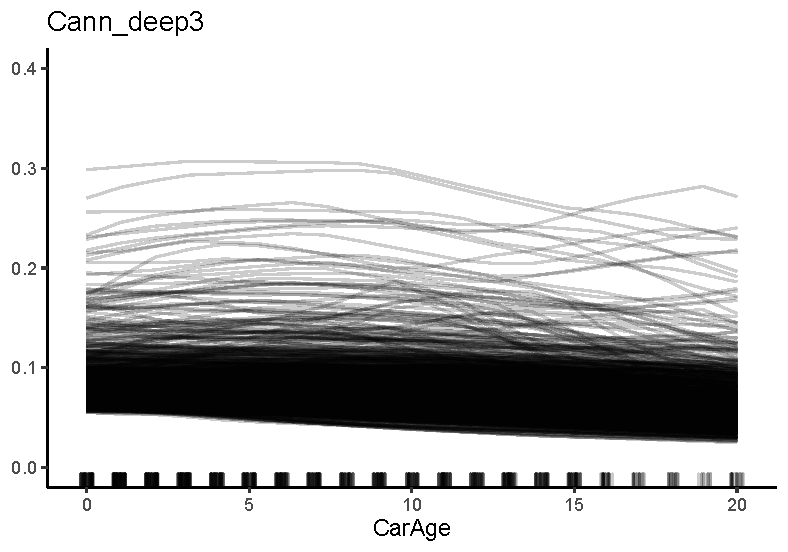
\includegraphics[scale=0.6]{Graphiques/iceCarCann}
\end{minipage}
\hfill
\begin{minipage}{0.45\linewidth}
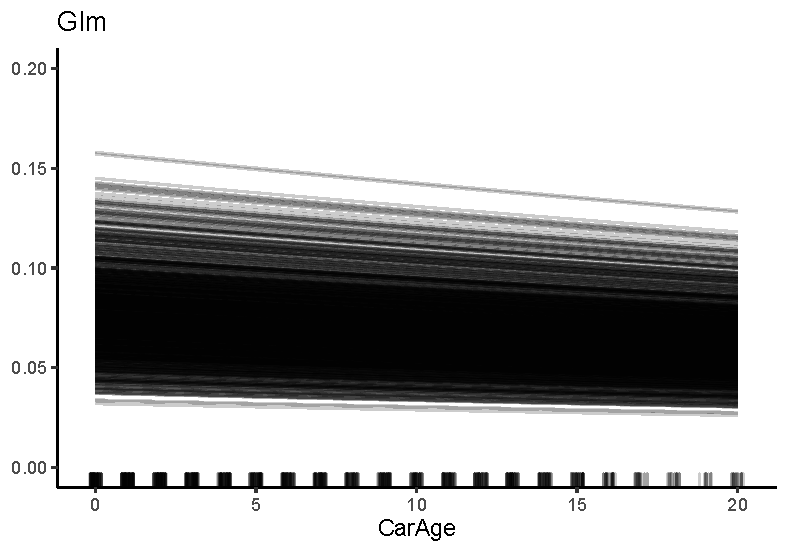
\includegraphics[scale=0.6]{Graphiques/iceCarGlm}
\end{minipage}
\end{figure}



L'effet de la variable \verb=Density= est plus difficile à distinguer. On voit clairement que la densité de la population fait augmenter le risque de réclammation pour ce portefeuille dans les trois modèles. Il semble avoir une légère différence pour le modèle CannDeep3 dans les extrémités de la courbe. Elle a une forme en « S », tandis que les deux autres courbes ne sont que convexes.

\begin{figure}
\centering
\caption{\label{fig:pdp3Density} Dépendance partielle pour la variable Density pour les trois modèles sélectionnés sur l'échelle logarithmique }
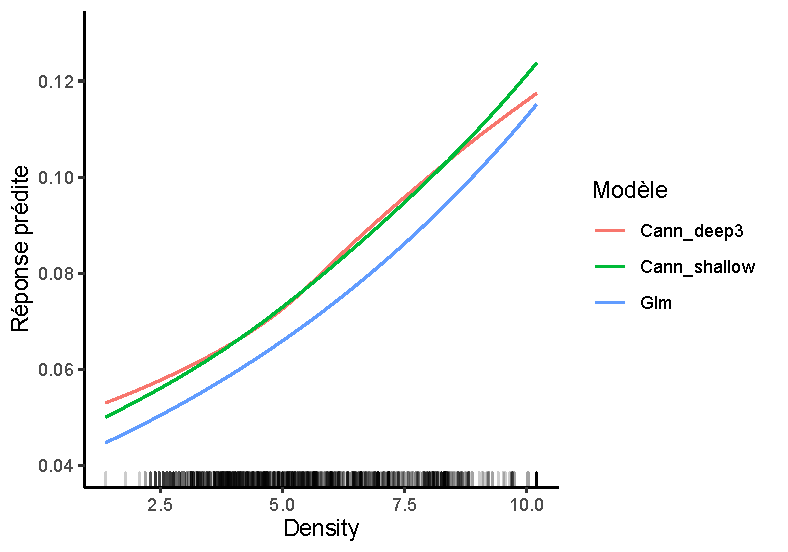
\includegraphics[scale=0.9]{Graphiques/pdp3ModDensity}
\end{figure}


La \autoref{fig:ice3Density} montre que le modèle CannDeep3 semble capter une interaction puisqu'on observe deux types de courbes. Le modèle prédit une légère augmentation pour une $log(Density)$ de 5 à 10 pour la plupart des assurés. Il y a cependant une certaine quantité d'assurés dont la prévision augmente rapidement pour des valeurs de 0 à 5 pour ensuite se stabiliser.

\begin{figure}
\caption{\label{fig:ice3Density} ICE pour la variable Density pour les trois modèles sélectionnés}
\centering
\begin{minipage}{0.45\linewidth}
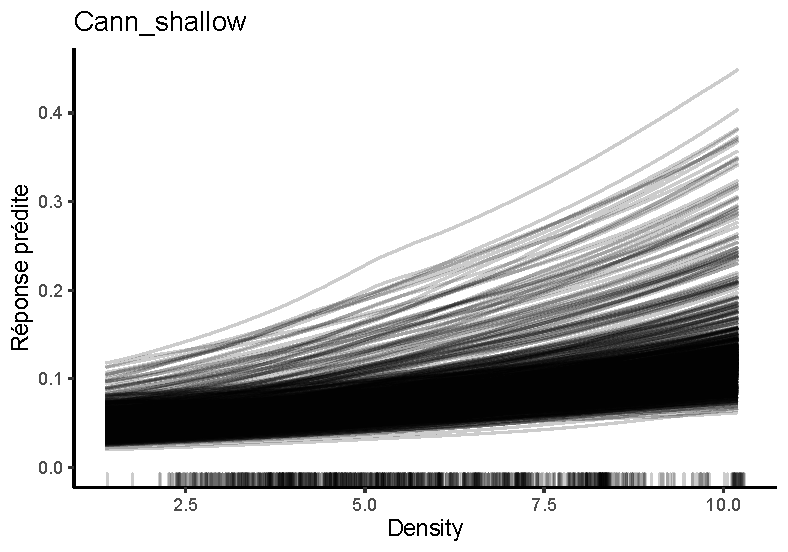
\includegraphics[scale=0.6]{Graphiques/iceDensityShallow}
\end{minipage}
\hfill
\begin{minipage}{0.45\linewidth}
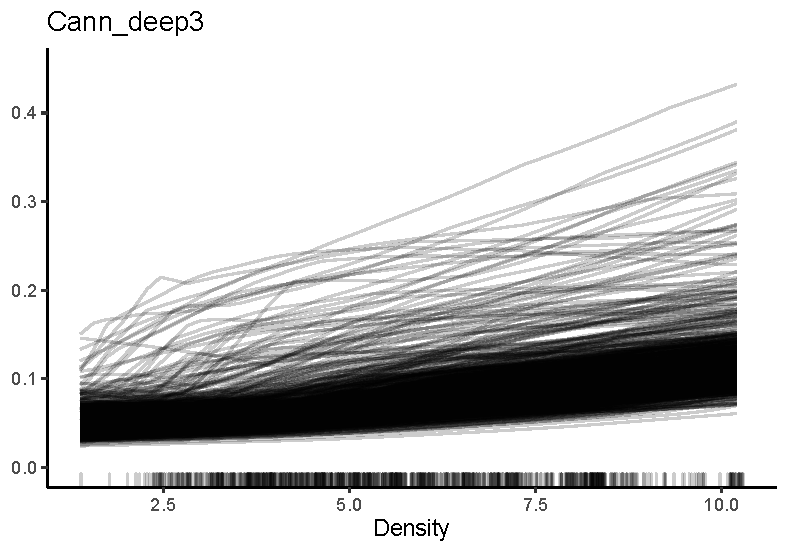
\includegraphics[scale=0.6]{Graphiques/iceDensityCann}
\end{minipage}
\hfill
\begin{minipage}{0.45\linewidth}
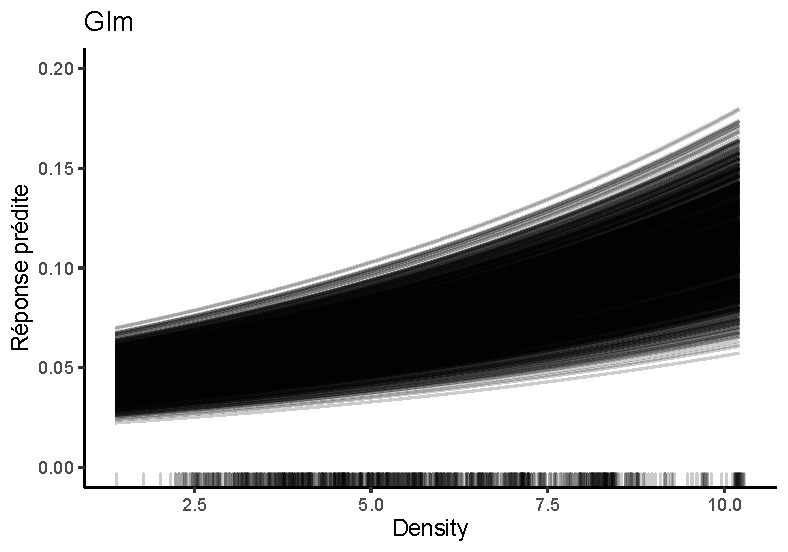
\includegraphics[scale=0.6]{Graphiques/iceDensityGlm}
\end{minipage}
\end{figure}


On observe à la \autoref{fig:interCann} que l'interaction de la variable \verb=Gas= avec les autres variables est la plus importante pour le modèle CannDeep3. Pour le modèle CannShallow, il s'agit de la variabe \verb=DriverAge=, \autoref{fig:interShallow}. On note plusieurs différences entre les deux modèles. Premièrement, le modèle CannDeep3 semble détecter plus d'interaction. Il y a cinq variables sur sept qui ont une statistique H supérieure à 0.2, tandis que le second réseau n'en compte que trois. Une autre différence notable est l'importance accordée aux interactions avec la variable \verb=DriverAge=. Le réseau profond la classe en cinquième position et le réseau à une couche la classe en première position. 


\begin{figure}
\centering
\caption{\label{fig:interCann} Interactions entre les variables explicatives pour le modèle CannDeep3 calculées à partir de la statistique H}
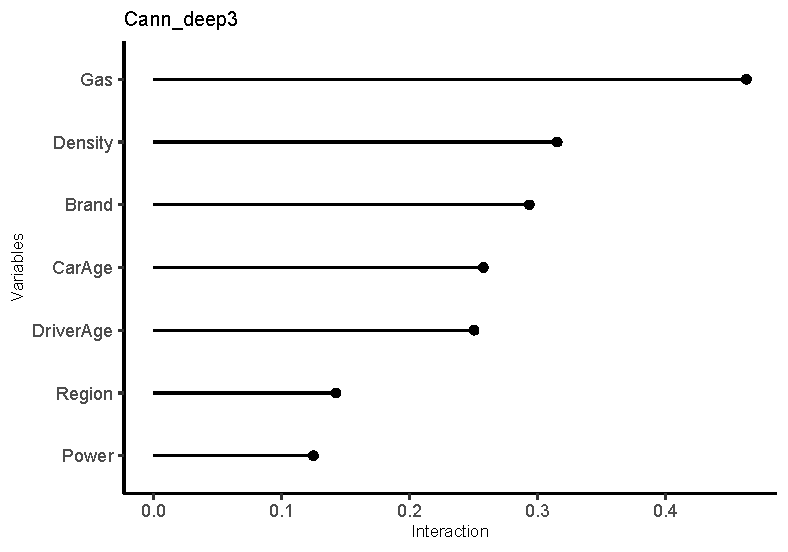
\includegraphics[scale=0.9]{Graphiques/interCann}
\end{figure}


\begin{figure}
\centering
\caption{\label{fig:interShallow} Interaction entre les variables explicatives pour le modèle CannShallow }
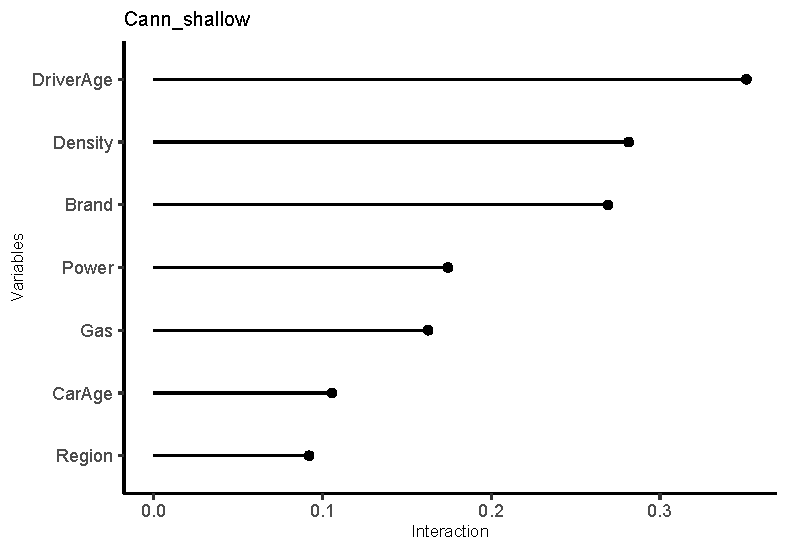
\includegraphics[scale=0.9]{Graphiques/interShallow}
\end{figure}

Les interactions avec la variable \verb=Gas= sont semblables pour les deux modèles. On note une seule différence notable pour l'interaction entre \verb=Density= et \verb=Gas=, où on obtient une statistique H à 0.2 pour le modèle CannDeep3 et 0.15 pour CannShallow.

\begin{figure}
\caption{\label{fig:inter3Gas} Interaction entre la variable Gas et les autres variables explicatives pour les modèles CannDeep3 et CannShallow}
\centering
\begin{minipage}{0.45\linewidth}
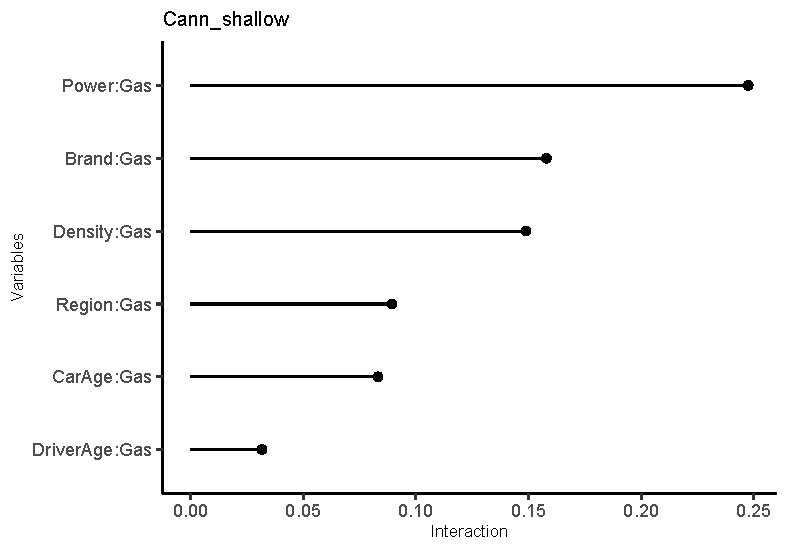
\includegraphics[scale=0.6]{Graphiques/interGasShallow}
\end{minipage}
\hfill
\begin{minipage}{0.45\linewidth}
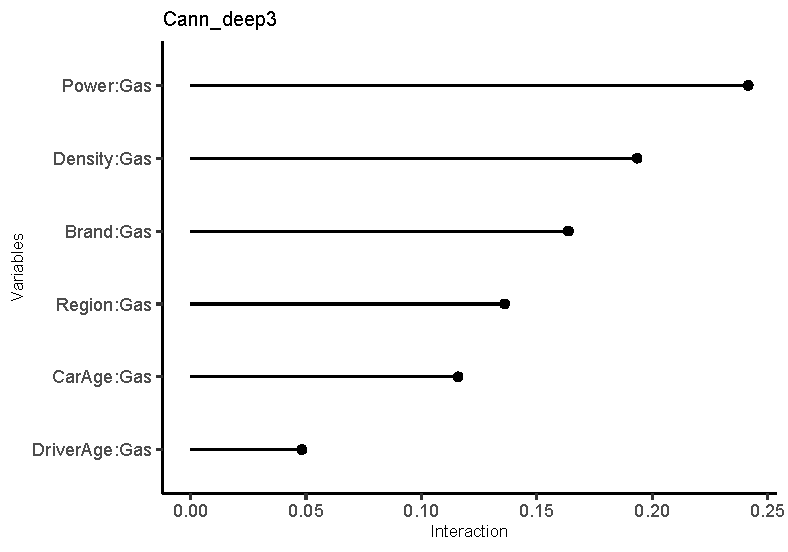
\includegraphics[scale=0.6]{Graphiques/interGasCann}
\end{minipage}
\end{figure}


On saisit mieux à l'aide de la \autoref{fig:inter3CarBrand} la raison possible de l'augmentation de la fréquence prédite des véhicules âgés de 5 à 10 ans par le modèle CannDeep3. On voit qu'il y a une interaction avec les véhicules japonnais. La courbe de cette marque de véhicule est clairement différente. Les autres marques ont toutes une diminution de la fréquence entre les âges mentionnés. Le réseau à une couche ne capte aucunement cet interaction. 

\begin{figure}
\caption{\label{fig:inter3CarBrand} Dépendance partielle entre les variables CarAge et Brand pour les trois modèles}
\centering
\begin{minipage}{0.45\linewidth}
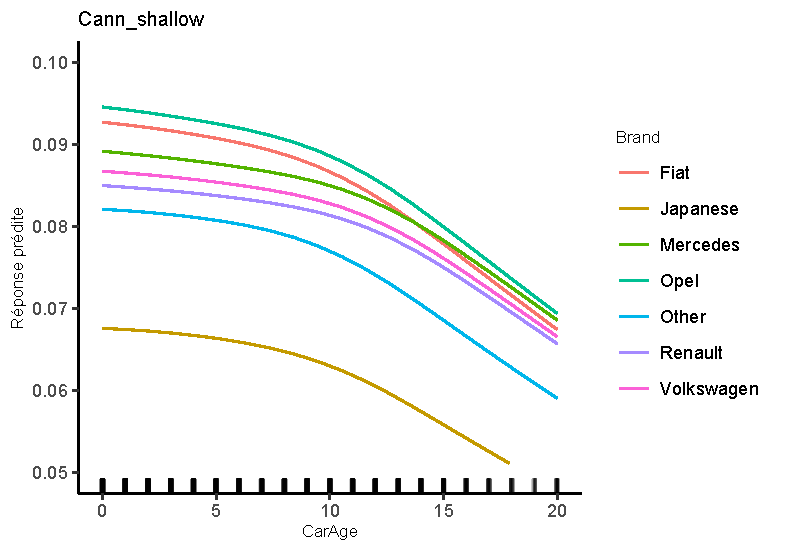
\includegraphics[scale=0.6]{Graphiques/interBrandCarShallow}
\end{minipage}
\hfill
\begin{minipage}{0.45\linewidth}
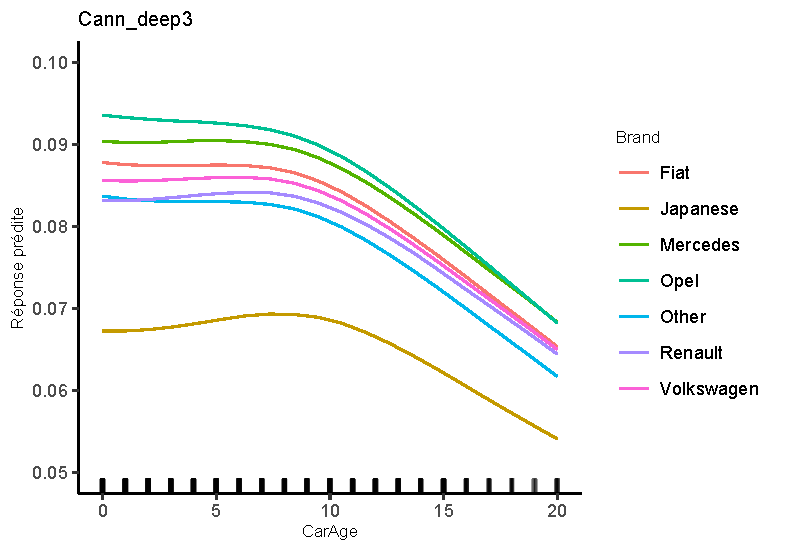
\includegraphics[scale=0.6]{Graphiques/interCarBrandCann}
\end{minipage}
\hfill
\begin{minipage}{0.45\linewidth}
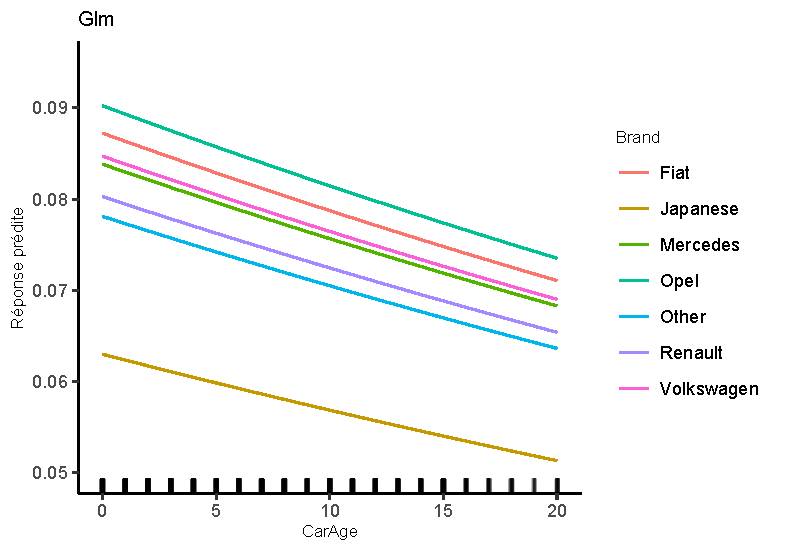
\includegraphics[scale=0.6]{Graphiques/interBrandCarGlm}
\end{minipage}
\end{figure}

On regarde maintenant les interactions avec \verb=DriverAge=. La \autoref{fig:inter3Driver} montre pour les deux modèles que les interactions avec \verb=Brand= et \verb=Density= sont les plus significatives. On illustre le PDP bivarié de \verb=DriverAge= et \verb=Density= à la \autoref{fig:inter3DriveDensity}. On y voit une différence pour les plus jeunes âges. Le modèles CannDeep3 prédit des fréquences élevées pour de jeunes conducteurs (environ moins de 25 ans) en combinaison avec une $log(Density)$ de 2.5 et plus. Le modèle CannShallow prédit des fréquences élevées pour de jeunes conducteurs, aussi, mais seulement pour une $log(Density)$ plus grande que 7.5 environ.

\begin{figure}
\caption{\label{fig:inter3Driver} Interaction entre la variable DriverAge et les autres variables explicatives pour les trois modèles}
\centering
\begin{minipage}{0.45\linewidth}
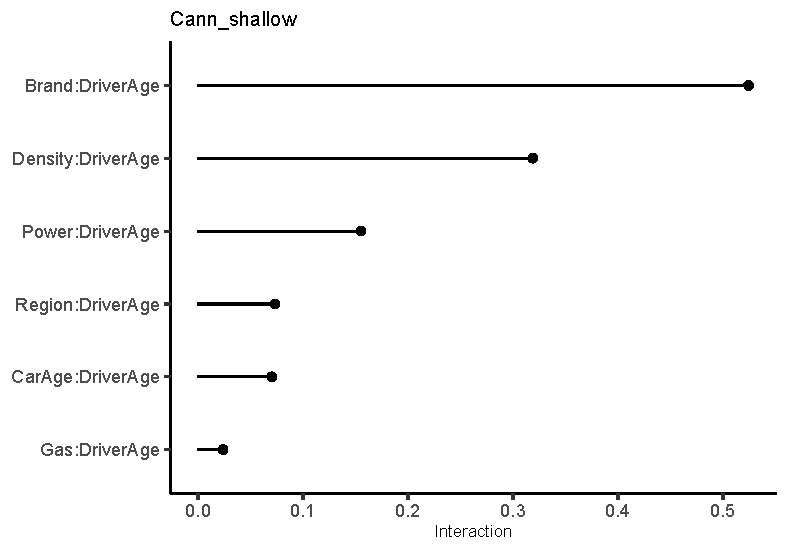
\includegraphics[scale=0.6]{Graphiques/interDriverAgeShallow}
\end{minipage}
\hfill
\begin{minipage}{0.45\linewidth}
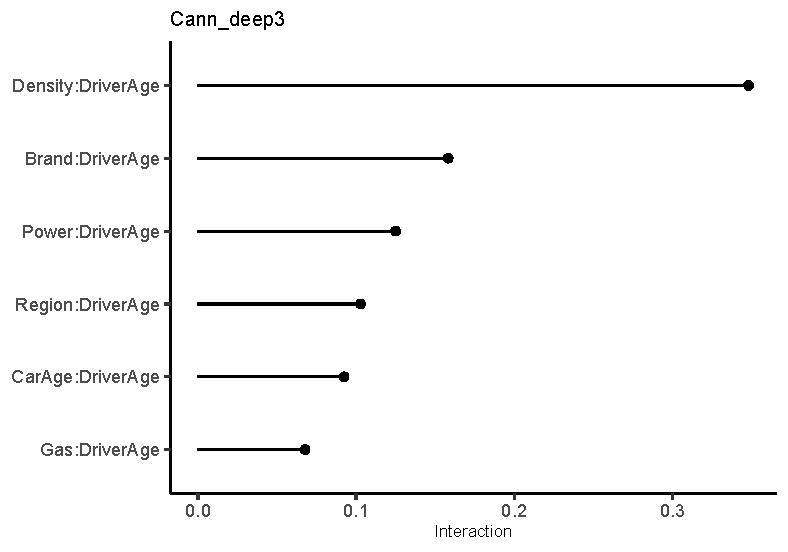
\includegraphics[scale=0.6]{Graphiques/interDriverAgeCann}
\end{minipage}
\end{figure}

\begin{figure}
\caption{\label{fig:inter3DriveDensity} Dépendance partielle entre les variables DriverAge et Density pour les trois modèles}
\centering
\begin{minipage}{0.45\linewidth}
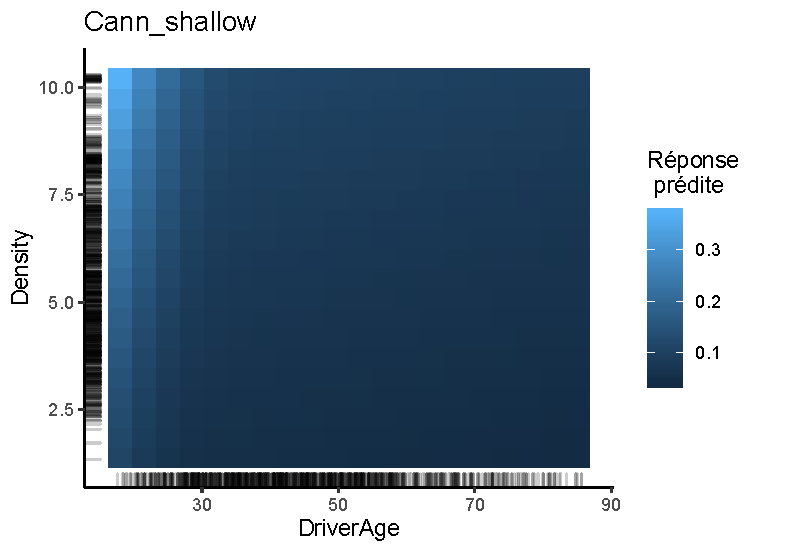
\includegraphics[scale=0.6]{Graphiques/interDriverDensityShallow}
\end{minipage}
\hfill
\begin{minipage}{0.45\linewidth}
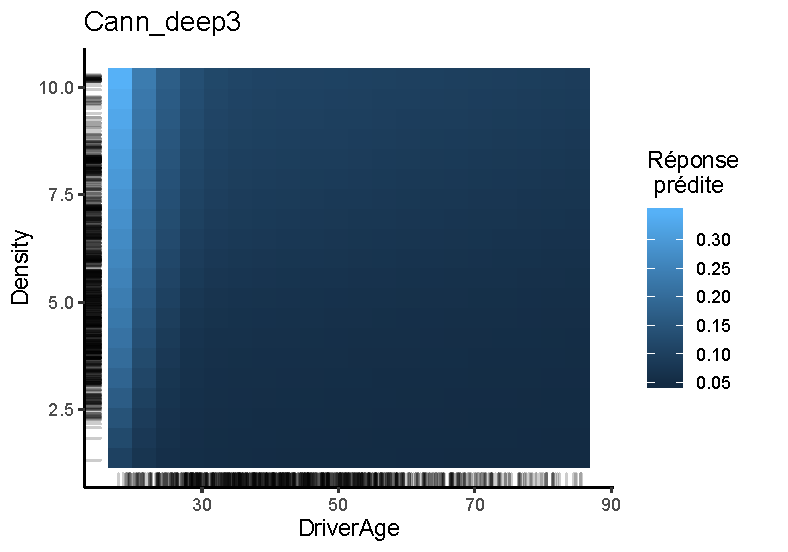
\includegraphics[scale=0.6]{Graphiques/interDriveDensityCann}
\end{minipage}
\hfill
\begin{minipage}{0.45\linewidth}
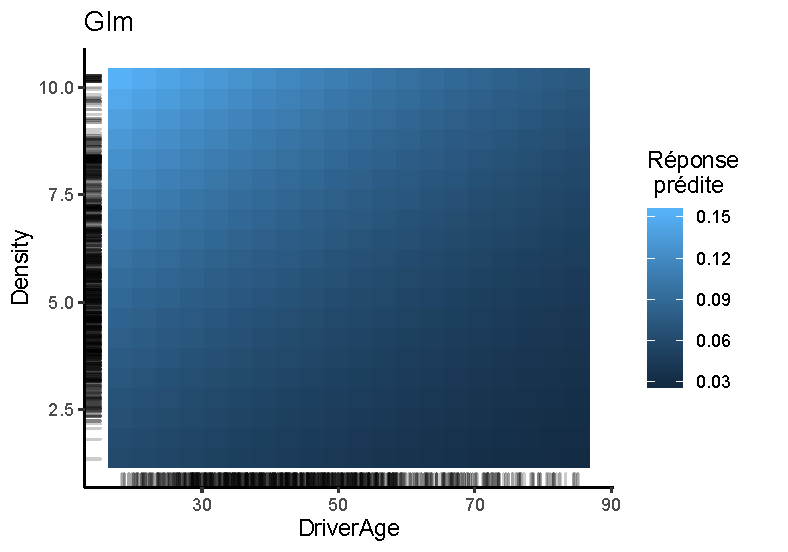
\includegraphics[scale=0.6]{Graphiques/interDriverDensityGlm}
\end{minipage}
\end{figure}           
\chapter*{Conclusion}           % ne pas numéroter
\label{chap:conclusion}         % étiquette pour renvois
\phantomsection\addcontentsline{toc}{chapter}{\nameref{chap:conclusion}} % inclure dans TdM

La dernière sous-section a permis de montrer que le modèle CannDeep3 a bien plus de facilité à découvrir les interactions. La combinaison entre sa structure et la façon d'initialiser le réseau aura permis de trouver un modèle performant de façon efficace. De plus, les résultats obtenus l'ont été à partir d'hyperparamètres optimisés pour des réseaux différents. On peut alors penser qu'ils bénéficieraient d'une recherche plus approfondie. Une autre avenue qui pourrait être étudiée est l'initialisation. Un modèle de base plus performant que celui utilisé pourrait permettre d'initialiser le réseau d'une meilleure façon encore. 

Cependant, la base de données simple et le problème peu compliqué ne sont peut-être pas la meilleure façon de tester l'utilité des réseaux de neurones en actuariat. Une des avenues possibles est l'utilisation de données massives comme les données télématiques d'automobiles pour modéliser la fréquence de réclamation comme \citet{gao2019claims} l'ont fait.
            % conclusion

\appendix                       % annexes le cas échéant

\chapter{Grilles de recherche}     % numérotée
\label{ann:grilleRecherche}                   


\begin{table}[h]
\centering
\caption{\label{tab:rechercheShallow} Grille de recherche pour le réseau « shallow » de 32 neurones}
\begin{tabular}{lc}
\toprule 
Hyperparamètre & Valeurs\\
\midrule
 $d$ & $\left\{0, 0.25, 0.5 \right\}$ \\ 
$\ell_1$  & $\left\{0 , 0.0001 \right\}$ \\ 
$\ell_2$  & $\left\{0 , 0.0001 \right\}$ \\ 
\bottomrule
 \end{tabular}  
\end{table}


\begin{table}[h]
\centering
\caption{\label{tab:rechercheDeep2} Grille de recherche pour le réseau à deux couches cachées}
\begin{tabular}{lc}
\toprule
Hyperparamètre  & Valeurs\\
\midrule
$d_1$ & $\left\{ 0, 0.25, 0.5 \right\}$\\
$d_2$ & $\left\{ 0, 0.25, 0.5 \right\}$\\
$\ell_1$ & $\left\{0, 0.0001 \right\}$\\
$\ell_2$ & $\left\{0, 0.0001 \right\}$\\
\bottomrule
\end{tabular}
\end{table}

\begin{table}[h]
\centering
\caption{\label{tab:rechercheDeep3} Grille de recherche pour le réseau à trois couches cachées}
\begin{tabular}{lc}
\toprule
Hyperparamètre  & Valeurs\\
\midrule
$d_1$ & $\left\{ 0,  0.25, 0.5 \right\}$\\
$d_2$ & $\left\{ 0, 0.25, 0.5 \right\}$\\
$\ell_1$ & $\left\{0, 0.00001 \right\}$\\
$\ell_2$ & $\left\{0, 0.00001 \right\}$\\
\bottomrule
\end{tabular}
\end{table}


\begin{table}[h]
\centering
\caption{\label{tab:rechercheDeep4} Grille de recherche pour le réseau à quatre couches cachées}
\begin{tabular}{lc}
\toprule
Hyperparamètre  & Valeurs\\
\midrule
$d_1$ & $\left\{ 0, 0.5 \right\}$\\
$d_2$ & $\left\{ 0, 0.5 \right\}$\\
$d_3$ & $\left\{ 0, 0.5 \right\}$\\
$\ell_1$ & $\left\{0, 0.000001 \right\}$\\
$\ell_2$ & $\left\{0, 0.000001 \right\}$\\
\bottomrule
\end{tabular}
\end{table}
\nocite{Hastie/etal:2009}
\nocite{wuthrich2019data}

\bibliography{Biblio}                 % production de la bibliographie

\end{document}
